\chapter{Schwarzschild black hole}
\label{s:sch}
\index{Schwarzschild!black hole}

\minitoc

\section{Introduction}

After having discussed stationary black holes in Chap.~\ref{s:sta},
we examine here the simplest of them: the Schwarzschild black hole.
Let us recall that the prime importance of this object
in general relativity stems from Israel uniqueness theorem
(Property~\ref{p:sta:Israel_uniqueness_thm}, Sec.~\ref{s:sta:no-hair}),
which states that any static black hole in an asymptotically flat 4-dimensional vacuum
spacetime ruled by general relativity must be a Schwarzschild black hole.

In this chapter, we derive the Schwarzschild metric as a solution to the
Einstein equation, possibly with a non-vanishing cosmological constant
$\Lambda$ (Sec.~\ref{s:sch:Sch_sol_lamb}); we then focus on the case $\Lambda=0$
(the true Schwarzschild solution) and explore it by means of the
Eddington-Finkelstein coordinates, which have
the advantage to be regular on the horizon (Sec.~\ref{s:sch:rad_geod_EF}).
Finally, in Sec.~\ref{s:sch:BH}, we check formally that the Schwarzschild spacetime has a region that obeys the general definition of a black hole given in
Sec.~\ref{s:glo:def_BH}. The maximal extension of the Schwarzschild
spacetime and its bifurcate Killing horizon
is discussed Chap.~\ref{s:max}, after two chapters (Chap.~\ref{s:ges} and \ref{s:gis})
devoted to the timelike and null geodesics in Schwarzschild
spacetime.

\section{The Schwarzschild-(anti-)de Sitter solution} \label{s:sch:Sch_sol_lamb}

\subsection{Vacuum Einstein equation with a cosmological constant}

Let us search for a static and spherically symmetric solution to the
Einstein equation (\ref{e:fra:vac_Einstein_Lambda}) in a vacuum
4-dimensional spacetime $(\M,\w{g})$ with some arbitrary cosmological constant
$\Lambda$. For $n=4$, Eq.~(\ref{e:fra:vac_Einstein_Lambda}) becomes
\be \label{e:sch:vac_Einstein_eq_Lamb}
    \encadre{ \w{R} = \Lambda \, \w{g} } .
\ee
An equivalent form is obtained by setting $\w{T}=0$
in the original Einstein equation (\ref{e:fra:Einstein_eq}):
\be \label{e:sch:vac_Einstein_eq}
    \encadre{ \w{R} + \left(\Lambda - \frac{1}{2}\, R\right)  \w{g} = 0 } .
\ee

\subsection{Static and spherically symmetric metric} \label{s:sch:static_spher}

Let us assume that the spacetime $(\M,\w{g})$ is \emph{static}\index{static!spacetime}, in the sense defined in Sec.~\ref{s:sta:def_station}:
the translation group $(\R,+)$ is a isometry group of $(\M,\w{g})$
(cf. Sec.~\ref{s:neh:symmetries}), with orbits that are timelike, at least near
some conformal boundary (stationarity property) and hypersurface-orthogonal (staticity property). Let us denote by $\w{\xi}$ the associated Killing vector
field (unique up to some constant rescaling), i.e. the generator of the
isometry group $(\R,+)$ (cf. Sec.~\ref{s:neh:symmetries}).

We may foliate $\M$ by a 1-parameter family of hypersurfaces
$\left(\Sigma_t\right)_{t\in\R}$, such that $\w{\xi}$ is normal to
all $\Sigma_t$'s and $t$ is a parameter associated to $\w{\xi}$:
\be \label{e:sch:xi_t}
    \w{\xi}(t) = 1
\ee
or equivalently, $\langle \dd t , \w{\xi} \rangle = 1$ [cf. Eq.~(\ref{e:sta:xi_wpar_t})].

In addition to being static, we assume that $(\M,\w{g})$ is \defin{spherically symmetric},
i.e. that it is invariant under the action of the rotation group $\mathrm{SO}(3)$,
whose orbits are spacelike 2-spheres (cf. Sec.~\ref{s:neh:symmetries}).
Let $\Sp$ be some generic 2-sphere orbit. The static Killing vector field $\w{\xi}$
must be orthogonal to $\Sp$, otherwise the orthogonal projection of $\w{\xi}$
onto $\Sp$ would define some privileged direction on $\Sp$, which is incompatible
with spherical symmetry. The orthogonality of $\w{\xi}$ and $\Sp$ implies
that $\Sp\subset\Sigma_t$. Let $(x^a)=(\th,\ph)$ be spherical coordinates on
$\Sp$. The (Riemannian) metric $\w{q}$ induced by $\w{g}$ on $\Sp$ is given by
\be
    \w{q} = r^2 \left( \dd\th^2 + \sin^2\th\, \dd\ph^2 \right) .
\ee
The positive coefficient $r^2$ in front of the standard spherical element must be
constant over $\Sp$, by virtue of spherical symmetry. The area of $\Sp$ is
then $A=4\pi r^2$. For this reason, $r$ is called the \defin{areal radius}\index{areal!radius}
of $\Sp$. Letting $\Sp$ vary, $r$ can be considered as a scalar field on
$\M$. If $\dd r \not = 0$, we may use it as a coordinate\footnote{An example of spherically symmetric spacetime with $\dd r = 0$ somewhere is the maximally extended Schwarzschild spacetime,
to be studied in Chap.~\ref{s:max}: $\dd r = 0$ on the so-called
\emph{bifurcation sphere}\index{bifurcation!sphere} $\Sp$ (cf. Sec.~\ref{s:max:bifur_Kill_hor}). Hence $r$ cannot be used
as a coordinate in the vicinity of $\Sp$; one shall use Kruskal-Szekeres coordinates instead.}. Since $\Sp\subset \Sigma_t$,
$(r,\th,\ph)$ is a coordinate system on each hypersurface $\Sigma_t$.
The set $(t,r,\th,\ph)$,
where $t$ is adapted to $\w{\xi}$ thanks to (\ref{e:sch:xi_t}), is then a
spacetime coordinate system and, by construction, the expression of the metric tensor
with respect to this system is
\be \label{e:sch:g_AB}
    \w{g} = -A(r)\, \dd t^2 + B(r)\, \dd r^2 +
        r^2 \left( \dd\th^2 + \sin^2\th\, \dd\ph^2 \right) .
\ee
Note that this is a special case of the general static metric element
(\ref{e:sta:static_metric}) and that Eq.~(\ref{e:sta:xi_wpar_t}) holds:
\be \label{e:sch:xi_wpar_t}
    \w{\xi} = \wpar_t .
\ee
In particular, $g_{tt} = -A(r)$ and $g_{rr} = B(r)$ do not depend on $t$
as a result of the spacetime stationarity, while
$g_{tr} = g_{t\th} = g_{t\ph} = 0$ expresses the orthogonality of $\w{\xi}$
and $\Sigma_t$, i.e. the spacetime staticity.
The coordinates $(t,r,\th,\ph)$ are called \defin{areal coordinates}\index{areal!coordinates},
reflecting the fact that $r$ is the areal radius.

\subsection{Solving the Einstein equation} \label{s:sch:solving_EE}

The Christoffel symbols of the metric (\ref{e:sch:g_AB}) with respect to the
areal coordinates are (cf. Sec.~\ref{s:sam:Kottler_solution} for the computation):
\be \label{e:sch:Christoffel_AB}
\begin{array}{l}
\displaystyle  \Gamma^t_{\ \, tr} = \Gamma^t_{\ \, rt} = \frac{1}{2A}\derd{A}{r}\qquad
\Gamma^r_{\ \, tt} = \frac{1}{2B}\derd{A}{r} \qquad
\Gamma^r_{\ \, rr} = \frac{1}{2B}\derd{B}{r} \qquad
\Gamma^r_{\ \, \th\th} = -\frac{r}{B} \\[2ex]
\displaystyle  \Gamma^r_{\ \, \ph\ph} = -\frac{r\sin^2\th}{B} \qquad
\Gamma^\th_{\ \, r\th} = \Gamma^\th_{\ \, \th r} = \frac{1}{r} \qquad
\Gamma^\th_{\ \, \ph\ph} = -\sin\th\cos\th \\[2ex]
\displaystyle \Gamma^\ph_{\ \, r\ph} = \Gamma^\ph_{\ \, \ph r} = \frac{1}{r} \qquad
\Gamma^\ph_{\ \, \th\ph} = \Gamma^\ph_{\ \, \ph\th} = \frac{1}{\tan\th} ,
\end{array}
\ee
the Christoffel symbols not listed above being zero.

The $tt$ component of the Einstein equation (\ref{e:sch:vac_Einstein_eq})
leads to (cf. Sec.~\ref{s:sam:Kottler_solution} for the computation)
\be \label{e:sch:EE_tt}
        r \derd{B}{r} - B + (1 - \Lambda r^2) B^2 = 0 ,
\ee
while the $rr$ component leads to
\be \label{e:sch:EE_rr}
        r \derd{A}{r} + A - (1 - \Lambda r^2) AB = 0 .
\ee
Finally, the $\th\th$ and $\ph\ph$ components lead to the same equation:
\be
    2  \frac{\D^2 A}{\D r^2} + \frac{2}{r} \derd{A}{r}
        - \frac{1}{B} \left( \derd{A}{r} + \frac{2A}{r} \right) \derd{B}{r}
        - \frac{1}{A} \left( \derd{A}{r} \right) ^2
        + 4 \Lambda  A B  = 0 .
\ee
All the other components of the Einstein equation (\ref{e:sch:vac_Einstein_eq})
are identically zero.

Adding Eq.~(\ref{e:sch:EE_tt}) multiplied by $A$ to
Eq.~(\ref{e:sch:EE_rr}) multiplied by $B$ yields
\[
    B \derd{A}{r} + A \derd{B}{r} = \derd{}{r}(AB) = 0 .
\]
The solution to this equation is obviously $A(r)B(r) = C$, where $C$ is a constant.
Without any loss of generality, we may choose $C=1$. Indeed, substituting
$C/B(r)$ for $A(r)$ in Eq.~(\ref{e:sch:g_AB}) results in
\[
    \w{g} = -\frac{C}{B(r)}\, \dd t^2 + B(r)\, \dd r^2 +
        r^2 \left( \dd\th^2 + \sin^2\th\, \dd\ph^2 \right) .
\]
Assuming $C>0$, the change of variable $t' = \sqrt{C} t$, which is equivalent
to changing the stationary Killing vector from $\w{\xi}$ to
$\w{\xi}'=  1/\sqrt{C}\, \w{\xi}$,
yields
\[
    \w{g} = -\frac{1}{B(r)}\, \dd t'^2 + B(r)\, \dd r^2 +
        r^2 \left( \dd\th^2 + \sin^2\th\, \dd\ph^2 \right) ,
\]
which is exactly the solution corresponding to $C=1$. Hence from now on,
we set $C=1$, i.e.
\be
    B(r) = \frac{1}{A(r)} .
\ee
Substituting this expression in Eq.~(\ref{e:sch:EE_rr}) yields an ordinary
differential equation for $A(r)$:
\[
    r \derd{A}{r} + A - 1 + \Lambda r^2 = 0 ,
\]
the solution to which is
\be
    A(r) = 1 - \frac{2 m}{r} - \frac{\Lambda}{3} \,  r^2 ,
\ee
where $m$ is a constant.
The general static and spherically symmetric solution to the vacuum
Einstein equation (\ref{e:sch:vac_Einstein_eq_Lamb}) is therefore
\be \label{e:sch:Kottler_metric}
    \encadre{
        \w{g} =
            -\left( 1 - \frac{2 m}{r} - \frac{\Lambda}{3} \,  r^2\right)\, \dd t^2
            + \left( 1 - \frac{2 m}{r} - \frac{\Lambda}{3} \,  r^2\right) ^{-1}\, \dd r^2+
        r^2 \left( \dd\th^2 + \sin^2\th\, \dd\ph^2 \right) }.
\ee
It is called the \defin{Kottler metric}\index{Kottler metric} (cf. the historical
note below).
The  \defin{Schwarzschild metric}\index{Schwarzschild!metric} is the
particular case $\Lambda=0$. If $\Lambda>0$,
(\ref{e:sch:Kottler_metric}) is called the
\defin{Schwarzschild-de Sitter metric}\index{Schwarzschild!de Sitter metric},
often abridged as \defin{Schwarzschild-dS metric}, while if $\Lambda<0$, it
is called the \defin{Schwarzschild-anti-de Sitter metric}\index{Schwarzschild!anti-de Sitter metric},
often abridged as \defin{Schwarzschild-AdS metric}\index{Schwarzschild!AdS metric}.

In the rest of this chapter, we will focus on the Schwarzschild metric,
i.e. on the version $\Lambda=0$ of Eq.~(\ref{e:sch:Kottler_metric}):
\be \label{e:sch:Schwarz_metric_SD}
    \encadre{
        \w{g} = -\left( 1 - \frac{2 m}{r} \right)\, \dd t^2
            + \left( 1 - \frac{2 m}{r} \right) ^{-1}\, \dd r^2 +
        r^2 \left( \dd\th^2 + \sin^2\th\, \dd\ph^2 \right) }.
\ee
The areal coordinates $(t,r,\th,\ph)$ are then called the
\defin{Schwarzschild-Droste coordinates}\index{Schwarzschild-Droste!coordinates}\footnote{In the literature they are often referred to as simply
\defin{Schwarzschild coordinates}\index{Schwarzschild!coordinates}; we follow
here Deruelle \& Uzan \cite{DerueU14,DerueU18}.}.

Since $A(r) = 1-2m/r$ and $B(r) = (1-2m/r)^{-1}$ for the Schwarzschild metric,
the non-vanishing Christoffel symbols (\ref{e:sch:Christoffel_AB})
become\footnote{See also the notebook \ref{s:sam:Kretschmann_Schwarz} for a
check.}
\be \label{e:sch:Christoffel_SD}
\begin{array}{l}
\displaystyle  \Gamma^t_{\ \, tr} = \Gamma^t_{\ \, rt} = \frac{m}{r(r-2m)}\qquad
\Gamma^r_{\ \, tt} = \frac{m(r-2m)}{r^3} \qquad
\Gamma^r_{\ \, rr} =  - \frac{m}{r(r-2m)}\\[2ex]
\displaystyle \Gamma^r_{\ \, \th\th} = 2m-r \qquad  \Gamma^r_{\ \, \ph\ph} = (2m -r)\sin^2\th \qquad
\Gamma^\th_{\ \, r\th} = \Gamma^\th_{\ \, \th r} = \frac{1}{r} \\[2ex]
\displaystyle \Gamma^\th_{\ \, \ph\ph} = -\sin\th\cos\th \qquad \Gamma^\ph_{\ \, r\ph} = \Gamma^\ph_{\ \, \ph r} = \frac{1}{r} \qquad
\Gamma^\ph_{\ \, \th\ph} = \Gamma^\ph_{\ \, \ph\th} = \frac{1}{\tan\th} .
\end{array}
\ee

\subsection{The mass parameter} \label{s:sch:mass_parameter}

The Schwarzschild metric (\ref{e:sch:Schwarz_metric_SD}) depends on a single
parameter: $m$. This parameter has a direct physical interpretation:
it is the \defin{gravitational mass}\index{mass!gravitational --}\index{mass!parameter of Schwarzschild solution} (or simply
\defin{mass}) that is felt by
an observer located at large values of $r$. Indeed, we will see in
Chap.~\ref{s:ges} that an observer on a circular orbit at a large value
of $r$ has an orbital period $T$ obeying Kepler's third law:
$T^2 = 4\pi^2 r^3 / m$. Without waiting for Chap.~\ref{s:ges}, we may notice
that for $r\gg |m|$, the metric (\ref{e:sch:Schwarz_metric_SD})
takes the standard weak-field form (see e.g. \cite{Carro04,MisneTW73}):
\be \label{e:sch:Schwarz_metric_large_r}
        \w{g} \simeq
            -\left( 1 + 2\Phi(r) \right) \, \dd t^2
            + \left( 1 - 2\Phi(r) \right)  \, \dd r^2 +
        r^2 \left( \dd\th^2 + \sin^2\th\, \dd\ph^2 \right) ,
\ee
where $\Phi(r) := -m/r$ is the Newtonian gravitational potential outside
a spherically symmetric body of mass $m$.

Another argument for identifying $m$ with a mass is provided by
Example~\ref{x:sta:Komar_mass_Schw} of Sec.~\ref{s:sta:Komar_mass}, where
it has been shown that $m$ is nothing but the \emph{Komar mass}\index{Komar!mass}\index{mass!Komar --} associated with the
stationarity of Schwarzschild spacetime.

\begin{hist} \label{h:sch:Schwarzschild_sol}
The Schwarzschild metric (\ref{e:sch:Schwarz_metric_SD}) is actually
the first non-trivial (i.e. different from Minkowski metric) exact solution
to the Einstein equation ever found. It has been obtained by the
astrophysicist Karl Schwarzschild\index[pers]{Schwarzschild, K.} in the end of 1915 \cite{Schwa1916}, only a few weeks
after the publication of the articles funding general relativity by
Albert Einstein\index[pers]{Einstein, A.}. It is also quite remarkable that
Schwarzschild found the solution while serving in the German army at the Russian
front. Unfortunately, he died from a rare skin disease a few months later.
The way Schwarzschild proceeded was quite different from that exposed above:
instead of the coordinates $(t,r,\th,\ph)$
named today after him, he used the coordinates
$(t,x^1,x^2,\ph)$ where $x^1 = r_*^3/3$, with $r_*^3 = r^3-8m^3$, and
$x^2 = -\cos\th$. Such a choice was made to enforce $\det(g_{\alpha\beta}) = -1$, a condition
prescribed by Einstein in an early version of general relativity, which had been presented on
18 November 1915 and on which Schwarzschild was working. Only in the final version, published on
25 November 1915, did Einstein relax the condition $\det(g_{\alpha\beta}) = -1$, allowing for full
covariance. Schwarzschild however
exhibited the famous metric (\ref{e:sch:Schwarz_metric_SD}), via what he
called the ``auxiliary quantity'' $r = (r_*^3 + 8m^3)^{1/3}$.
For him, the ``center'',  namely the location of the ``point mass'' generating the field,
was at $r_* = 0$, i.e. at $r=2m$.
Independently of Schwarzschild, Johannes Droste\index[pers]{Droste, J.}, then PhD student of
Hendrik Lorentz\index[pers]{Lorentz, H.},
arrived at the solution (\ref{e:sch:Schwarz_metric_SD}) in May 1916 \cite{Drost1917}.
Contrary to Schwarzschild, Droste performed the computation with
a spherical coordinate system, $(t,\bar r, \th,\ph)$, yet distinct from
the standard ``Schwarzschild-Droste'' coordinates $(t,r,\th,\ph)$ by the fact that the radial
coordinate $\bar r$ was not chosen to be the areal radius, but instead a
coordinate for which $g_{\bar r\bar r} = 1$. At the end, by a change of
variable, Droste exhibited the metric (\ref{e:sch:Schwarz_metric_SD}).
The generalization to a non-vanishing cosmological constant, i.e.
Eq.~(\ref{e:sch:Kottler_metric}), has been obtained by
Friedrich Kottler\index[pers]{Kottler, F.} in 1918 \cite{Kottl1918} and, independently, by
Hermann Weyl\index[pers]{Weyl, H.} in 1919 \cite{Weyl1919}. We refer to Eisenstaedt's article
\cite{Eisen82} for a detailed account of the early history of the
Schwarzschild solution.
\end{hist}


\subsection{The Schwarzschild-Droste domain} \label{s:sch:SD_domain}

We immediately notice on (\ref{e:sch:Schwarz_metric_SD}) that the metric
components are singular at $r=0$ and $r=2m$. Accordingly, the Schwarzschild-Droste coordinates $(t,r,\th,\ph)$ cover the following subset of $\M$, which we call the
\defin{Schwarzschild-Droste domain}\index{Schwarzschild-Droste!domain}:
\begin{subequations}
\begin{align}
    \M_{\rm SD} & :=  \M_{\rm I} \cup \M_{\rm II} , \\
    \M_{\rm I} & :=  \R\times(2m,+\infty)\times\SS^2 ,\\
    \M_{\rm II} & :=  \R\times(0,2m)\times\SS^2 ,
\end{align}
\end{subequations}
with the coordinate $t$ spanning $\R$, the coordinate $r$ spanning $(2m,+\infty)$
on $\M_{\rm I}$ and $(0,2m)$ on $\M_{\rm II}$, and the coordinates $(\th,\ph)$
constituting a standard spherical chart of $\SS^2$.
Note that $\M_{\rm SD}$ is a disconnected open subset of the full spacetime
manifold $\M$ (to be specified later), whose connected components are
$\M_{\rm I}$ and $\M_{\rm II}$.

\begin{remark}
To cover entirely $\SS^2$ in a regular way, one needs a second chart, in
addition to $(\th,\ph)$; this is related to the standard singularities of
spherical coordinates at $\th=0$ and $\th=\pi$. It is fully understood
that the metric $\w{g}$, as expressed by (\ref{e:sch:Schwarz_metric_SD}), is
fully regular on $\SS^2$. The fact that $\det(g_{\alpha\beta}) = -r^2\sin^2\th$ is zero
at $\th=0$ and $\th=\pi$ reflects merely the coordinate singularity
of the $(\th,\ph)$ chart there. We shall not discuss this coordinate singularity
any further.
\end{remark}

The boundary value $r_{\rm S}:= 2m$ of $r$ between $\M_{\rm I}$ and $\M_{\rm II}$
is conventionaly called the \defin{Schwarzschild radius}\index{Schwarzschild!radius}.
A more appropriate name would have been the \emph{Schwarzschild areal radius},
for $r$ does not describe a \emph{radius} (in the sense of a distance from
some ``origin'') but rather an \emph{area}, as discussed in Sec.~\ref{s:sch:static_spher}.

Immediate properties of the Schwarzschild-Droste domain are:

\begin{prop}[the Schwarzschild exterior $\M_{\rm I}$]
Region $(\M_{\rm I}, \w{g})$ is strictly static, in the sense defined in
Sec.~\ref{s:sta:def_station}: the Killing vector $\w{\xi} = \wpar_t$ is
timelike on all $\M_{\rm I}$ and is orthogonal to the hypersurfaces $t= \mathrm{const}$.
Moreover, $(\M_{\rm I}, \w{g})$ is asymptotically flat: the metric $\w{g}$ tends to Minkowski metric
when $r\rightarrow +\infty$.
\end{prop}

\begin{proof}
From expression (\ref{e:sch:Schwarz_metric_SD}), we see that $g_{tt} < 0$ for $r > 2 m$.
Since $g_{tt} = \w{g}(\wpar_t, \wpar_t)$, this implies that $\wpar_t$ is timelike.
Moreover $\wpar_t$ is orthogonal to any hypersurface $\Sigma_t$ defined by a constant
value of $t$, since we read on (\ref{e:sch:Schwarz_metric_SD}) that
$\w{g}(\wpar_t, \wpar_i) = g_{ti} = 0$ for $i\in\{1,2,3\}$ and by definition,
the vectors $(\wpar_i) = (\wpar_r,\wpar_\th,\wpar_\ph)$ form a basis of the tangent planes to $\Sigma_t$.
Finally, for $r\to +\infty$, all the metric components given by (\ref{e:sch:Schwarz_metric_SD})
tend to those of the Minkowksi metric (\ref{e:glo:Mink_metric_spher})
[see also Eq.~(\ref{e:sch:Schwarz_metric_large_r})].
\end{proof}

\begin{prop}[the Schwarzschild interior $\M_{\rm II}$]
\label{p:sch:prop_M_II}
In region $\M_{\rm II}$, the Killing vector $\w{\xi} = \wpar_t$ is spacelike.
It follows that $(\M_{\rm II},\w{g})$ is \emph{not} static:
the translation group $(\R,+)$ is still an
isometry group of $(\M_{\rm II},\w{g})$, but its orbits are spacelike curves
(cf. Sec.~\ref{s:sta:def_station}).
Besides, in $\M_{\rm II}$, $t$ is a spacelike coordinate
(i.e. the hypersurfaces $t=\mathrm{const}$ are timelike, cf. Sec.~\ref{s:bas:signature})
and $r$ is a timelike one (i.e. the hypersurfaces $r=\mathrm{const}$ are spacelike).
\end{prop}

\begin{proof}
We see from (\ref{e:sch:Schwarz_metric_SD}) that $g_{tt} > 0$ for $r< 2m$,
which implies that $\wpar_t$ is spacelike there.
Moreover, we have $g^{tt} > 0$ and $g^{rr} < 0$ in
$\M_{\rm II}$, which, according to the criterion~(\ref{e:bas:char_causal_type_coord}),
implies that $t$ is a spacelike coordinate
and $r$ a timelike one.
\end{proof}

\begin{remark}
In the region $\M_{\rm II}$, $g_{rr} < 0$, so that the
metric $\w{g}$ keeps a Lorentzian signature, as it should!
\end{remark}

\begin{remark}
As a consequence of Property~\ref{p:sch:prop_M_II} and of the diagonal character of
the metric components (\ref{e:sch:Schwarz_metric_SD}),
the axes of the light cones are horizontal lines for $r<2m$ in Fig.~\ref{f:sch:rad_null_geod} below.
\end{remark}

%%%%%%%%%%%%%%%%%%%%%%%%%%%%%%%%%%%%%%%%%%%%%%%%%%%%%%%%%%%%%%%%%%%%%%%%%%%%%%%

\section{Radial null geodesics and Eddington-Finkelstein coordinates}
\label{s:sch:rad_geod_EF}

\subsection{Radial null geodesics}
\label{s:sch:rad_null_geod}

Let us search for the null geodesics of the Schwarzschild metric
(\ref{e:sch:Schwarz_metric_SD}) that are radial, i.e. along which
$\th=\mathrm{const}$ and $\ph=\mathrm{const}$. They are found by
setting  $\D\th=0$ and $\D\ph=0$ in the line element (\ref{e:fra:line_element})
and searching for $\D s^2 = g_{\mu\nu}\, \D x^\mu \, \D x^\nu = 0$,
with the $g_{\mu\nu}$'s read on (\ref{e:sch:Schwarz_metric_SD}):
\be \label{e:sch:radial_null}
    \D s^2 = 0 \iff \D t^2 = \frac{\D r^2}{\left( 1 - \frac{2m}{r} \right) ^2} .
\ee
Hence the radial null geodesics are governed by
\be \label{e:sch:Dt_Dr_radial_null_geod}
    \D t = \pm \frac{\D r}{ 1 - \frac{2m}{r} } .
\ee
This equation is easily integrated:
\be \label{e:sch:t_r_radial_null_geod}
    t = \pm \left( r + 2 m \ln \left| \frac{r}{2m} - 1 \right| \right) + \mathrm{const} .
\ee
We have thus two families of curves, one for each choice
of the sign $\pm$:

\begin{figure}
\centerline{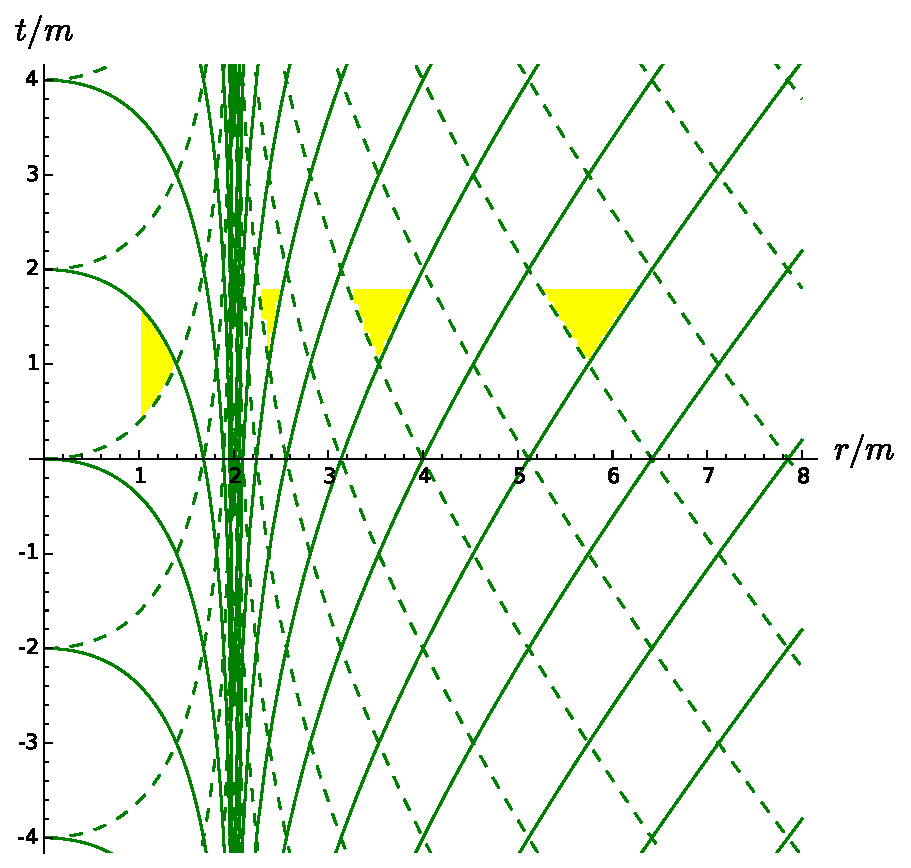
\includegraphics[width=0.6\textwidth]{sch_rad_null_geod.pdf}}
\caption[]{\label{f:sch:rad_null_geod} \footnotesize
Radial null geodesics of Schwarzschild spacetime, plotted in terms
of Schwarzschild-Droste coordinates $(t,r)$: the solid (resp. dashed) lines
correspond to outgoing (resp. ingoing) geodesics $\Li^{\rm out}_{(u,\th,\ph)}$
(resp. $\Li^{\rm in}_{(v,\th,\ph)}$), as given by Eq.~(\ref{e:sch:outgoing_null_geod})
(resp. Eq.~(\ref{e:sch:ingoing_null_geod})). The interiors of some future light
cones are depicted in yellow.}
\end{figure}

\begin{itemize}
\item the \defin{outgoing radial null geodesics}\index{outgoing!null geodesic}
$\Li^{\rm out}_{(u,\th,\ph)}$, whose
equation is
\be \label{e:sch:outgoing_null_geod}
   \Li^{\rm out}_{(u,\th,\ph)}:\quad
   \encadre{ t = r + 2 m \ln \left| \frac{r}{2m} - 1 \right| + u },
\ee
where $u\in \R$ is a constant along $\Li^{\rm out}_{(u,\th,\ph)}$;
\item  the \defin{ingoing radial null geodesics}\index{ingoing!null geodesic}
$\Li^{\rm in}_{(v,\th,\ph)}$, whose
equation is
\be \label{e:sch:ingoing_null_geod}
 \Li^{\rm in}_{(v,\th,\ph)}:\quad  \encadre{ t = - r - 2 m \ln \left| \frac{r}{2m} - 1 \right| + v },
\ee
where $v\in \R$ is a constant along $\Li^{\rm in}_{(v,\th,\ph)}$.
\end{itemize}
Note that along a given outgoing radial null geodesic, $(u,\th,\ph)$ are constant and that
two outgoing radial null geodesics that have distinct $(u,\th,\ph)$ are distinct. We can thus
use the triplet $(u,\th,\ph)$ to label the outgoing radial null geodesics,
leading to the notation $\Li^{\rm out}_{(u,\th,\ph)}$. Moreover, the family $(\Li^{\rm out}_{(u,\th,\ph)})$,
with $u\in\R$, $\th\in[0,\pi]$ and $\ph \in [0, 2\pi)$, %]$
forms a \defin{congruence}\index{congruence}: there is one, and only one, such curve through
every point of $\M_{\rm SD}$. Similar considerations apply to the ingoing radial null geodesics
$\Li^{\rm in}_{(v,\th,\ph)}$.

By introducing the \defin{tortoise coordinate}\index{tortoise coordinate}
\be \label{e:sch:def_tortoise}
    r_* := r + 2 m \ln \left| \frac{r}{2m} - 1 \right| ,
\ee
one may rewrite Eqs.~(\ref{e:sch:outgoing_null_geod})-(\ref{e:sch:ingoing_null_geod}) as
respectively
\bea
  \Li^{\rm out}_{(u,\th,\ph)}:\quad  &  & t = r_* + u \\
  \Li^{\rm in}_{(v,\th,\ph)}:\quad  &  & t = -r_* + v . \label{e:sch:v_advanced_tortoise}
\eea
The parameter $u$ appears then as a
\defin{retarded time}\index{retarded!time}\index{time!retarded --}:
$u = t - r_*$ and $v$ as an
\defin{advanced time}\index{advanced!time}\index{time!advanced --}: $v = t + r_*$.

Strictly speaking, we have found radial null \emph{curves} only, i.e. solutions of
Eq.~(\ref{e:sch:radial_null}). Since not all null curves
are null geodesics\footnote{A famous counterexample is the null helix in Minkowski
spacetime, cf. Remark~\ref{r:def:null_curves} on p.~\pageref{r:def:null_curves}.}, there remains to prove that the curves defined
by (\ref{e:sch:outgoing_null_geod}) and (\ref{e:sch:ingoing_null_geod})
obey the geodesic equation\index{geodesic!equation} [Eq.~(\ref{e:geo:eq_geod}) in Appendix~\ref{s:geo}]:
\be \label{e:sch:geod_eqn}
    \frac{\D^2 x^\alpha}{\D \lambda^2} + \Gamma^\alpha_{\ \, \mu\nu}
        \derd{x^\mu}{\lambda} \derd{x^\nu}{\lambda} = 0 ,
\ee
where $\lambda$ is an affine parameter (cf. Sec.~\ref{s:geo:def}).
Let us check that (\ref{e:sch:geod_eqn}) is satisfied by choosing $\lambda=r$.
For the curves defined by (\ref{e:sch:outgoing_null_geod}), we have
\[
   \left( x^\alpha(r) \right) = \left( r + 2 m \ln \left| \frac{r}{2m} - 1 \right| + u,\ r,\  \th,\  \ph \right) .
\]
Hence
\[
    \left( \derd{x^\alpha}{r} \right) = \left( \frac{r}{r-2m}, 1, 0, 0 \right)
    \qquad\mbox{and}\qquad
    \left(  \frac{\D^2 x^\alpha}{\D r^2} \right) = \left( - \frac{2m}{(r-2m)^2}, 0, 0, 0 \right) .
\]
Given the Christoffel symbols (\ref{e:sch:Christoffel_SD}), it is then a
simple exercise to show that Eq.~(\ref{e:sch:geod_eqn}) is satisfied.
The same property holds for the family (\ref{e:sch:ingoing_null_geod}). Hence
we conclude
\begin{prop}[radial null geodesics]
\label{p:sch:radial_null_geod}
The radial null geodesics in the Schwarzschild-Droste domain
form two congruences, $(\Li^{\rm out}_{(u,\th,\ph)})$ and $(\Li^{\rm in}_{(v,\th,\ph)})$,
obeying Eqs.~(\ref{e:sch:outgoing_null_geod})-(\ref{e:sch:ingoing_null_geod}).
Moreover, the areal radius $r$ is an affine parameter along them.
\end{prop}

The two congruences of radial null geodesics are depicted in
Fig.~\ref{f:sch:rad_null_geod}.
The singularity of Schwarzschild-Droste coordinates at
the Schwarzschild radius $r=2m$
appears clearly on this figure.


\begin{remark} \label{r:sch:outgoing_ingoing}
Despite their name, geodesics of the outgoing family $\Li^{\rm out}_{(u,\th,\ph)}$ are actually
\emph{ingoing} in the region $r<2m$, in the sense that
$r$ is decreasing along them when moving towards the future. Indeed,
as noticed in Sec.~\ref{s:sch:SD_domain},
for $r<2m$, $\wpar_r$ is a timelike vector and we shall see in Sec.~\ref{s:sch:time_orientation}
that $-\wpar_r$ is oriented towards the future (cf. the ``tilted'' light cone
in Fig.~\ref{f:sch:rad_null_geod}).
\end{remark}

\subsection{Eddington-Finkelstein coordinates} \label{s:sch:EF_coord}

The parameter $v$ is one of the three parameters labelling the
ingoing radial null geodesics $\Li^{\rm in}_{(v,\th,\ph)}$.
Let us promote it to a spacetime coordinate, instead of $t$, i.e. let us
consider the coordinate system $(v,r,\th,\ph)$ that is related to the
Schwarzschild-Droste coordinates $(t,r,\th,\ph)$ by Eq.~(\ref{e:sch:ingoing_null_geod}):
\be \label{e:sch:v_t_r}
     v = t + r + 2 m \ln \left| \frac{r}{2m} - 1 \right| .
\ee
By differentiation, it follows immediately that
\be \label{e:sch:dt_dv_NIEF}
    \dd t = \dd v -  \frac{\dd r}{1 - 2m/r} ,
\ee
the tensor square of which is [cf. Eq.~(\ref{e:bas:sym_tensor_prod})]
\[
    \dd t^2 = \dd v^2 - \frac{2}{1 - 2m/r} \, \dd v \, \dd r + \frac{1}{(1 - 2m/r)^2}\, \dd r^2 .
\]
Substituting this expression for $\dd t^2$ in Eq.~(\ref{e:sch:Schwarz_metric_SD})
yields the metric components with respect to the coordinates
$(x^{\hat{\alpha}}) := (v,r,\th,\ph)$:
\be \label{e:sch:Schwarz_metric_NIEF}
    \encadre{
        \w{g} =
            -\left( 1 - \frac{2 m}{r} \right)\, \dd v^2
            + 2 \, \dd v \, \dd r
        + r^2 \left( \dd\th^2 + \sin^2\th\, \dd\ph^2 \right) }.
\ee

\begin{remark}
Since $\dd v\, \dd r := 1/2 \, (\dd v\otimes \dd r +  \dd r\otimes\dd v)$
[cf. Eq.~(\ref{e:bas:sym_tensor_prod})], the metric component $g_{vr}$
is \emph{one half} of the coefficient of the $\dd v\, \dd r$ term
in Eq.~(\ref{e:sch:Schwarz_metric_NIEF}), i.e.
$g_{vr} = 1$.
\end{remark}

The coordinates $(x^{\hat{\alpha}}) = (v,r,\th,\ph)$ are called the
\defin{null ingoing Eddington-Finkelstein (NIEF) coordinates}\index{Eddington-Finkelstein!coordinates}\index{null!ingoing Eddington-Finkelstein coordinates}\index{NIEF}. The qualifier \emph{null} stems from the fact that
$v$ is a null coordinate\index{null!coordinate}, i.e. the level sets $v = \mathrm{const}$ are null hypersurfaces
(cf. Sec.~\ref{s:bas:signature}). This can be seen from $g^{vv} = 0$ [cf. Eq.~(\ref{e:bas:char_causal_type_coord})].

To deal with a timelike coordinate instead of a null one, let us set
\be  \label{e:sch:ti_v_r}
    \encadre{\ti := v - r} \iff \encadre{v = \ti + r}
\ee
and define the \defin{ingoing Eddington-Finkelstein (IEF) coordinates}\index{Eddington-Finkelstein!coordinates}\index{ingoing!Eddington-Finkelstein!coordinates}\index{IEF}
to be
\be
    (x^{\tilde{\alpha}}) := (\ti, r, \th,\ph) .
\ee

\begin{remark}
From (\ref{e:sch:ti_v_r}), $v$ appears as the ``time'' $\ti$ ``advanced'' by
$r$\index{advanced!time}\index{time!advanced --}, while
from (\ref{e:sch:v_advanced_tortoise}), $v$ is the ``time'' $t$ ``advanced''
by $r_*$.
\end{remark}

The relation between the ingoing Eddington-Finkelstein coordinates
$(\ti, r, \th,\ph)$
and the Schwarzschild-Droste ones $(t,r,\th,\ph)$ is obtained by combining
Eqs.~(\ref{e:sch:v_t_r}) and (\ref{e:sch:ti_v_r}):
\be \label{e:sch:ti_t_r}
     \encadre{\ti = t + 2 m \ln \left| \frac{r}{2m} - 1 \right| } .
\ee
The hypersurfaces $t=\mathrm{const}$ are plotted in Fig.~\ref{f:sch:SD_slices},
in terms of the IEF coordinates.

\begin{figure}
\centerline{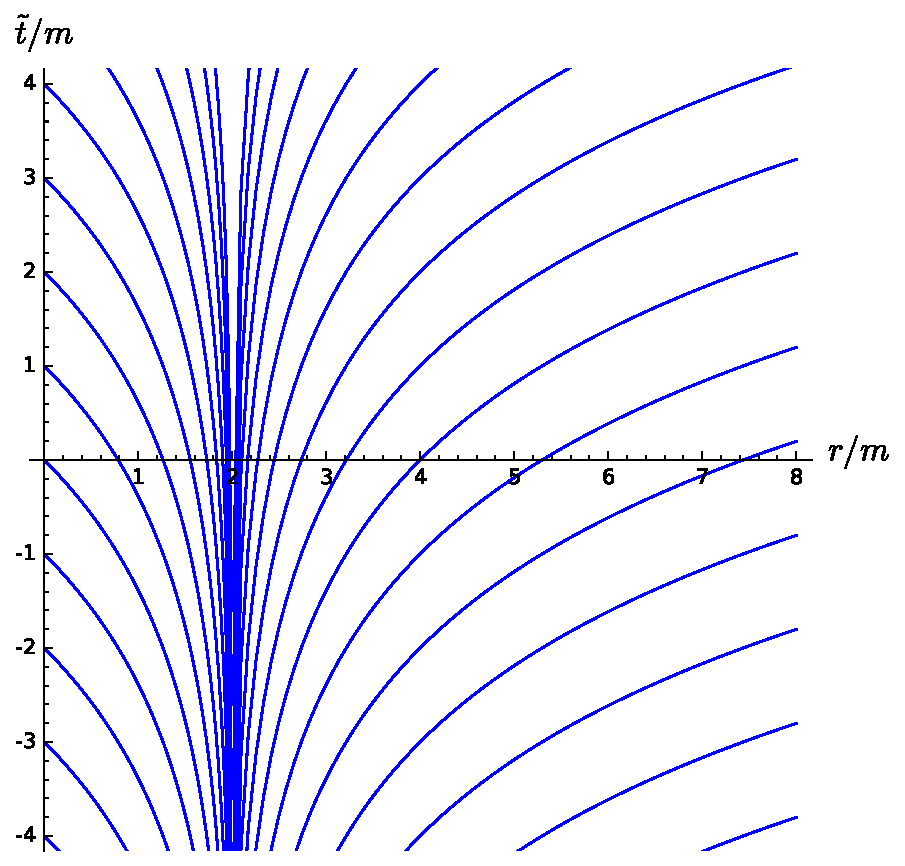
\includegraphics[width=0.6\textwidth]{sch_SD_slices.pdf}}
\caption[]{\label{f:sch:SD_slices} \footnotesize
Hypersurfaces of constant Schwarzschild-Droste coordinate $t$, drawn in terms
of the ingoing Eddington-Finkelstein coordinates $(\ti,r)$. Since the dimensions
along $\th$ and $\ph$ are not represented, these 3-dimensional surfaces appear
as curves.}
\end{figure}

From (\ref{e:sch:ti_v_r}), we have $\dd v = \dd\ti + \dd r$. Substituting
into (\ref{e:sch:Schwarz_metric_NIEF}) yields
\be \label{e:sch:Schwarz_metric_EF}
    \encadre{
        \w{g} =
            -\left( 1 - \frac{2 m}{r} \right)\, \dd \ti^2
            + \frac{4m}{r} \, \dd \ti \, \dd r
            + \left( 1 + \frac{2 m}{r} \right)\, \dd r^2
        + r^2 \left( \dd\th^2 + \sin^2\th\, \dd\ph^2 \right) }.
\ee

To avoid any ambiguity, we shall denote by $\wpar_{\tilde{r}}$ the
coordinate vector of the IEF frame and by
$\wpar_r$ the coordinate vector of the Schwarzschild-Droste frame:
\be
    \wpar_{\tilde{r}} := \left. \der{}{r} \right| _{\ti,\th,\ph}
    \qquad\mbox{and}\qquad
    \wpar_r := \left. \der{}{r} \right| _{t,\th,\ph} .
\ee
The relation between the two vectors is given by the chain rule:
\[
    \left. \der{}{r} \right| _{\ti,\th,\ph}  =
    \left. \der{}{t} \right| _{r,\th,\ph}
    \underbrace{ \left. \der{t}{r} \right| _{\ti,\th,\ph}}_{\left(1-\frac{r}{2m}\right)^{-1}}
  + \left. \der{}{r} \right| _{t,\th,\ph}
   \underbrace{\left. \der{r}{r} \right| _{\ti,\th,\ph}}_{1}
  + \left. \der{}{\th} \right| _{t,r,\ph}
  \underbrace{\left. \der{\th}{r} \right| _{\ti,\th,\ph}}_{0}
  + \left. \der{}{\ph} \right| _{t,r,\th}
  \underbrace{\left. \der{\ph}{r} \right| _{\ti,\th,\ph}}_{0} ,
\]
where (\ref{e:sch:ti_t_r}) has been used to evaluate
$\left. \dert{t}{r} \right| _{\ti,\th,\ph}$. Hence
\be \label{e:sch:wpar_tilde_r}
    \wpar_{\tilde{r}} = \wpar_r + \left(1-\frac{r}{2m}\right)^{-1} \, \wpar_t .
\ee

On the other hand, we deduce from (\ref{e:sch:ti_t_r}) that
\[
     \left. \der{}{\ti} \right| _{r,\th,\ph} = \left. \der{}{t} \right| _{r,\th,\ph} ,
\]
which implies:
\be  \label{e:sch:wpar_tilde_t}
    \wpar_{\ti} = \wpar_t .
\ee
In particular, the vector $\wpar_{\ti}$ of the IEF frame coincides with
the Killing vector $\w{\xi}$:
\be \label{e:sch:wparti_xi}
    \encadre{ \wpar_{\ti} = \w{\xi}} .
\ee
\begin{remark}
The result (\ref{e:sch:wparti_xi}) is not surprising since
the metric components (\ref{e:sch:Schwarz_metric_EF}) are independent from
$\ti$. This implies that $\wpar_{\ti}$ is a Killing vector. $\ti$ being a timelike coordinate in $\M_{\rm I}$, it
follows that $\wpar_{\ti} = \alpha \w{\xi}$, where $\alpha$ is a constant.
Since $\ti \sim t$ when $r\rightarrow +\infty$, we get $\alpha=1$.
\end{remark}

\begin{remark}
In region $\M_{\rm II}$,
the four vectors $(\wpar_{\ti},\wpar_{\tilde{r}}, \wpar_\th, \wpar_\ph)$
are spacelike\footnote{This follows from the diagonal components $g_{\alpha\alpha}$
read on (\ref{e:sch:Schwarz_metric_EF}) being positive for $r<2m$,
but this can also be seen
graphically on Fig.~\ref{f:sch:rad_null_geod_EF} below: for $r<2m$,
both the $\ti$ and $r$ coordinate lines, i.e. the vertical and horizontal lines,
are outside the light cones.}. There is nothing wrong about that; in particular this does not
contradict the signature $(-,+,+,+)$ of the metric. The latter is related
to the type of the basis vectors only when the metric components take
a \emph{diagonal} form, which is not the case here, since
$g_{\ti r} \neq 0$ [Eq.~(\ref{e:sch:Schwarz_metric_EF})].
All that is demanded
to $(\ti,r,\th,\ph)$ for being (locally) a regular coordinate system is that
$(\wpar_{\ti},\wpar_{\tilde{r}}, \wpar_\th, \wpar_\ph)$ form a basis of
the tangent space $T_p\M$ at each point $p$. This can be achieved with any causal type
of the vectors $(\wpar_{\ti},\wpar_{\tilde{r}}, \wpar_\th, \wpar_\ph)$.
\end{remark}

\begin{remark}
The IEF expression (\ref{e:sch:Schwarz_metric_EF}) for the metric can be recast
in the following remarkable form:
\be \label{e:sch:Kerr_Schild}
  \w{g} =
 \underbrace{- \dd\ti^2 + \dd r^2 + r^2  \left( \dd\th^2 + \sin^2\th\,
   \dd\ph^2 \right)}_{\w{f}}
 + \frac{2m}{r} \underbrace{\left( \dd\ti + \dd r \right) ^2}_{\uu{k}\otimes\uu{k}} ,
\ee
where the $\w{f}$ is the (flat) Minkowski metric (expressed above in
terms of the spherical coordinates $(\ti,r,\th,\ph)$) and $\uu{k} = - \dd(\ti + r) = - \dd v$.
The 1-form $\uu{k}$ is dual to a vector $\w{k}$, which is null, as it can be seen
from
$g^{\tilde{\mu}\tilde{\nu}} k_{\tilde{\mu}} k_{\tilde{\nu}} = 0$. The latter property
is easily deduced from
$k_{\tilde{\mu}} = (-1, -1, 0, 0)$ and expression (\ref{e:sch:inv_metric_EF})
for $g^{\tilde{\mu}\tilde{\nu}}$ below.
A metric of the type (\ref{e:sch:Kerr_Schild}) is said to be a
\defin{Kerr-Schild metric}\index{Kerr-Schild!metric}; these peculiar metrics
are discussed in Appendix~\ref{s:ksm}.
\end{remark}

\begin{hist} \label{n:sch:Eddington_coord}
Eddington-Finkelstein coordinates have been introduced by
Arthur Eddington\index[pers]{Eddington, A.} in 1924 \cite{Eddin1924}. More precisely, Eddington
introduced the \emph{outgoing} version of these coordinates,
while we have focused above on the \emph{ingoing} version. Indeed
Eddington's Eq.~(2) is $\ti = t - 2m \ln(r-m)$, which mainly differs from
our Eq.~(\ref{e:sch:ti_t_r}) by the minus sign in front of the logarithm\footnote{The other differences with (\ref{e:sch:ti_t_r}) are a constant additive term
and a misprint in Eddington's formula: the term $\ln(r-m)$ should be replaced
by $\ln(r-2m)$.},
which means that Eddington's time coordinate is actually $\ti = u + r$, instead of
$\ti = v - r$ (our Eq.~(\ref{e:sch:ti_v_r})). Eddington used his transformation
to get the Kerr-Schild form (\ref{e:sch:Kerr_Schild}) of Schwarzschild metric,
with $(\D \ti + \D r)^2$ replaced by $(\D \ti - \D r)^2$ due to the change
ingoing $\leftrightarrow$ outgoing. For a modern reader, it is quite surprising
that Eddington did not point out that the metric components w.r.t. $(\ti,r,\th,\ph)$
are regular at $r=2m$. Actually the main purpose of Eddington's article
\cite{Eddin1924} was elsewhere, in the comparison of general relativity to an alternative theory proposed in 1922 by the mathematician Alfred N. Whitehead
(see e.g. \cite{GibboW08}).
Only in 1958 did David Finkelstein\index[pers]{Finkelstein, D.} reintroduce the Eddington transformation
and conclude that the Schwarzschild metric is analytic over the whole domain
$r\in(0,+\infty)$ \cite{Finke58}. Meanwhile the regularity of Schwarzschild metric
at $r=2m$ had been proven by Georges Lemaître\index[pers]{Lemaitre, G.@Lemaître, G.} in 1932 \cite{Lemai32}, via
another coordinate system, which we shall introduce in
Sec.~\ref{s:lem:Schwarzschild} (see also \cite{Eisen93} for a detailed discussion),
as well as by John Synge\index[pers]{Synge, J.L.} in 1950 \cite{Synge50}, by means of yet another coordinate
system (cf. the historical note on p.~\pageref{n:max:KS_coord}).
\end{hist}

\begin{remark}
In the literature, the terminology \emph{Eddington-Finkelstein coordinates}
is often used for the coordinates $(v,r,\th,\ph)$ (or $(u,r,\th,\ph)$),
i.e. for what we have called the \emph{null Eddington-Finkelstein coordinates},
and the regularity of the metric tensor at $r=2m$ is demonstrated by
considering the components (\ref{e:sch:Schwarz_metric_NIEF}).
However, neither
Eddington \cite{Eddin1924} nor Finkelstein \cite{Finke58}
considered this null version: they used coordinates $(\ti,r,\th,\ph)$
and they exhibited (the outgoing version of) the
metric components (\ref{e:sch:Schwarz_metric_EF}).
Hence our terminology is more faithful to history.
\end{remark}




\subsection{The Schwarzschild horizon} \label{s:sch:Schwarz_hor}

Contrary to the Schwarzschild-Droste components (\ref{e:sch:Schwarz_metric_SD}),
the metric components (\ref{e:sch:Schwarz_metric_EF}) are regular as
$r\rightarrow 2m$. Hence
(\ref{e:sch:Schwarz_metric_EF}) defines a regular non-degenerate metric
on the whole \defin{ingoing Eddington-Finkelstein domain}\index{ingoing!Eddington-Finkelstein!domain}
\be \label{e:sch:M_IEF_def}
    \M_{\rm IEF} := \R\times(0,+\infty)\times\SS^2,
\ee
with the coordinate $\ti$ spanning $\R$, the coordinate $r$ spanning
$(0,+\infty)$ and the coordinates $(\th,\ph)$ forming the standard spherical
chart of $\SS^2$.
The components of the inverse metric with respect to the IEF coordinates are
\be \label{e:sch:inv_metric_EF}
    g^{\tilde{\alpha}\tilde{\beta}} = \left( \begin{array}{cccc}
    - \left( 1 + \frac{2m}{r} \right) &  \frac{2m}{r} & 0 & 0 \\[1ex]
    \frac{2m}{r} & 1 - \frac{2m}{r} & 0 & 0 \\[1ex]
    0 & 0 & \frac{1}{r^2} & 0 \\[1ex]
    0 & 0 & 0 & \frac{1}{r^2\sin^2\th}
    \end{array} \right) .
\ee
In particular, the components $g^{\tilde{\alpha}\tilde{\beta}}$ are regular at $r=2m$.
Moreover we notice that $g^{\ti\ti} < 0$ for all $r\in(0,+\infty)$. In view of
the criterion~(\ref{e:bas:char_causal_type_coord}), we may assert

\begin{prop}[Timelike character of the IEF coordinate $\ti$]
\label{p:sch:ti_timelike}
The coordinate $\ti$ is timelike in all $\M_{\rm IEF}$.
\end{prop}
This is in contrast with the Schwarzschild-Droste coordinate $t$, which is
timelike in $\M_{\rm I}$ but spacelike
in $\M_{\rm II}$ (Property~\ref{p:sch:prop_M_II}).


The IEF domain is an extension of the Schwarzschild-Droste domain
introduced in Sec.~\ref{s:sch:SD_domain}:
\be
    \M_{\rm IEF} = \M_{\rm SD} \cup \Hor = \M_{\rm I} \cup \M_{\rm II} \cup \Hor ,
\ee
where $\Hor$ is the subset of $\M_{\rm IEF}$ defined by $r=2m$. Note that
$\Hor$ has the topology
\be
    \Hor \simeq \R\times\SS^2
\ee
and that $(\ti,\th,\ph)$ is a coordinate system on $\Hor$.
Actually $\Hor$ is nothing but what has been called the
\defin{Schwarzschild horizon}\index{Schwarzschild!horizon} in the examples
of Chaps.~\ref{s:def} and \ref{s:neh}. Indeed, the metric
(\ref{e:sch:Schwarz_metric_EF}) is nothing but
the metric (\ref{e:def:Schw_metric}) introduced in Example~\ref{x:def:Schw_hor}
of Chap.~\ref{s:def} (p.~\pageref{x:def:Schw_hor}), up to the change of notation $\ti \leftrightarrow t$ (compare (\ref{e:def:Schw_metric_inv}) and
(\ref{e:sch:inv_metric_EF}) as well).
We have thus the fundamental result,
the proof of which is given in Example~\ref{x:neh:Schwarz_KH} of Chap.~\ref{s:neh}
(p.~\pageref{x:neh:Schwarz_KH}):
\begin{prop}
The hypersurface $\Hor$ defined by $r=2m$
is a Killing horizon, the null normal of which is $\w{\xi}$.
\end{prop}
In particular, $\Hor$ is a null hypersurface, whose null geodesic generators
admit $\w{\xi} = \wpar_{\ti}$ as tangent vector. It is a non-expanding horizon,
whose area, as defined in Sec.~\ref{s:neh:invar_area}, is (cf. Example~\ref{x:neh:Schwarz_hor_area} of Chap.~\ref{s:neh}, p.~\pageref{x:neh:Schwarz_hor_area})
\be
    A=16\pi m^2 .
\ee
$\Hor$ is depicted in Fig.~\ref{f:def:Schwarz_horizon}.
We shall see in Sec.~\ref{s:sch:BH} that $\Hor$ is actually a
black hole event horizon in Schwarzschild spacetime.

\begin{hist}
The first author to recognize that the hypersurface $r=2m$ in Schwarzschild spacetime
is a one-way membrane, i.e. a horizon, is David Finkelstein\index[pers]{Finkelstein, D.}
in 1958~\cite{Finke58}. Amazingly, Finkelstein stressed rather $r=2m$
as a \emph{white hole} boundary in a time-reversed version of $(\M_{\rm IEF},\w{g})$. In particular, he
wrote \emph{``causal influences propagating into the "future" can cross the Schwarzschild surface only
in an outward direction''} (see also his Fig.~1). The reason is that Finkelstein considered
the extension of the $\M_{\rm I}$ region to $r\leq 2m$ constructed with
the \emph{outgoing}
coordinate $\tilde{\tilde t} = t - 2 m \ln ( {r}/(2m) - 1 )$ [his Eq.~(2.3) in our notations] instead of $\ti$ as given by Eq.~(\ref{e:sch:ti_t_r}). However, he noticed that another
extension of $\M_{\rm I}$ can be obtained by time inversion,
corresponding to a \emph{``surface that is permeable inwards''}. As we shall see in Chap.~\ref{s:max},
both black hole and white hole regions actually exist in the maximal extension
of Schwarzschild spacetime.
\end{hist}


\subsection{Coordinate singularity vs. curvature singularity}
\label{s:sch:singularities}

The above considerations show that the divergence of the metric
component $g_{rr}$ in (\ref{e:sch:Schwarz_metric_SD}) when $r\rightarrow 2m$
reflects a pathology of Schwarzschild-Droste coordinates and not a singularity
in the metric tensor $\w{g}$ by itself: $(\M_{\rm IEF}, \w{g})$ is perfectly
regular spacetime, including at the Schwarzschild radius $r=2m$.
The bad behavior of Schwarzschild-Droste coordinates is obvious in Fig.~\ref{f:sch:SD_slices}: the hypersurfaces
$t=\mathrm{const}$ fail to provide a regular slicing of spacetime.
This pathology is called a
\defin{coordinate singularity}\index{coordinate!singularity}\index{singularity!coordinate --}, since it is intrinsic a given coordinate system
(here the Schwarzschild-Droste one).

Another pathology appears in the metric components in both the Schwarzschild-Droste coordinates and the ingoing Eddington-Finkelstein ones: $g_{tt}$ and $\tilde{g}_{\ti\ti}$ diverge when $r\rightarrow 0$. This type of singularity
cannot be removed by a coordinate transformation. Indeed, the
\defin{Kretschmann scalar}\index{Kretschmann scalar}, defined as the
following ``square'' of the Riemann curvature tensor
\be \label{e:sch:def_Kretschmann}
    K := R_{\mu\nu\rho\sigma} R^{\mu\nu\rho\sigma} ,
\ee
is\index{Kretschmann scalar!of Schwarzschild metric} (cf. Sec.~\ref{s:sam:Kretschmann_Schwarz} for the computation)
\be \label{e:sch:value_Kretschmann}
    K = \frac{48 m^2}{r^6} .
\ee
Hence $K\rightarrow +\infty$ when $r\rightarrow 0$. Since $K$ is a scalar
field, its value is independent of any coordinate system used to express it.
Hence the divergence of $K$ reflects a pathology of the Riemann tensor
per se: it is called a
\defin{curvature singularity}\index{curvature!singularity}\index{singularity!curvature --}.
Physically, this means that unbounded tidal forces\index{tidal force} are felt by any system
approaching $r=0$. This interpretation holds because
tidal forces correspond to
the acceleration of the separation vector between
neighboring timelike geodesics and that acceleration is
governed by the Riemann tensor,
via the \emph{geodesic deviation equation}\index{geodesic!deviation equation}\index{deviation!geodesic --}, cf. Property~\ref{p:geo:geod_deviation} (see Chap.~11 of MTW \cite{MisneTW73} for more details).


\begin{figure}
\centerline{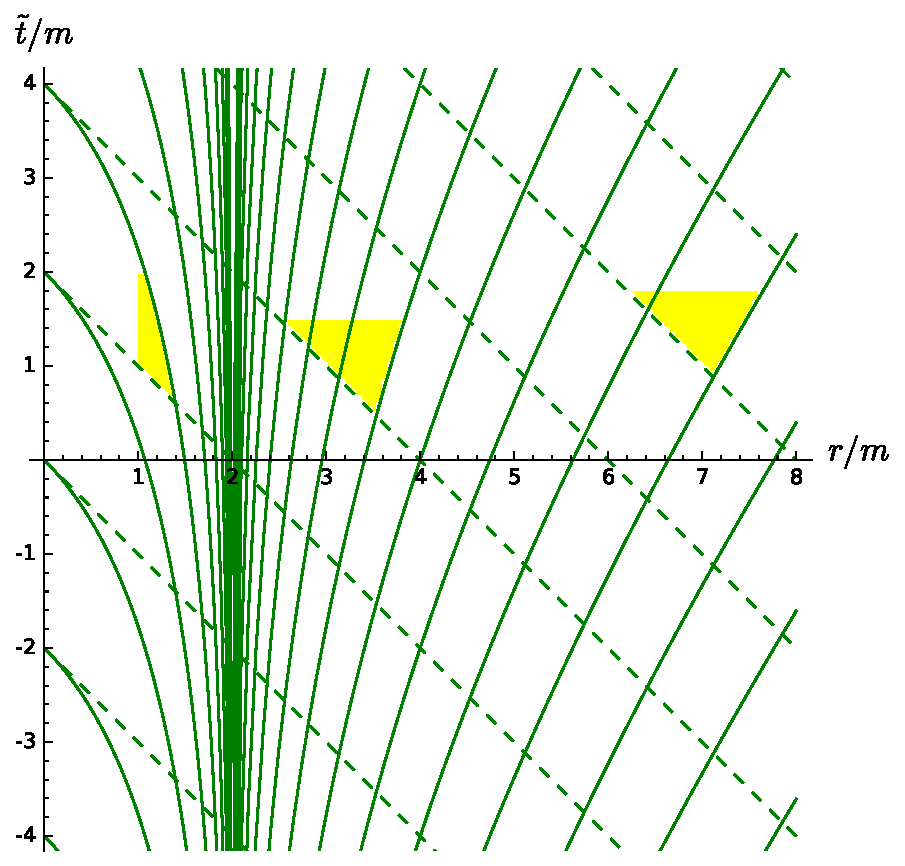
\includegraphics[width=0.6\textwidth]{sch_rad_null_geod_EF.pdf}}
\caption[]{\label{f:sch:rad_null_geod_EF} \footnotesize
Radial null geodesics of Schwarzschild spacetime, plottved in terms
of ingoing Eddington-Finkelstein coordinates $(\ti,r)$: the solid (resp. dashed) lines
correspond to outgoing (resp. ingoing) geodesics $\Li^{\rm out}_{(u,\th,\ph)}$
(resp. $\Li^{\rm in}_{(v,\th,\ph)}$), as given by Eq.~(\ref{e:sch:outgoing_null_geod_EF})
(resp. Eq.~(\ref{e:sch:ingoing_null_geod_EF})). The interiors of some future light
cones are depicted in yellow. Note that the hypersurfaces of constant $\ti$
(horizontal lines) always lie outside the light cones, i.e. are spacelike, in agreement with
$\ti$ being everywhere a timelike coordinate (Property~\ref{p:sch:ti_timelike}).
Similarly the hypersurfaces of constant $r$ (vertical lines) lie outside the light cones
for $r<2m$, in agreement with $r$ being a timelike coordinate in $\M_{\rm II}$
(Property~\ref{p:sch:prop_M_II}).}
\end{figure}

\subsection{Radial null geodesics in terms of the Eddington-Finkelstein coordinates}
\label{s:sch:radial_null_IEF}

Let us search directly for the radial null geodesics on the IEF domain $\M_{\rm IEF}$
by looking for the radial null curves of the metric (\ref{e:sch:Schwarz_metric_EF}).
The vanishing of the line element $\D s^2 = \w{g}(\D\w{x},\D\w{x})$ for the
radial displacement $\D\w{x} = \D\ti \, \wpar_{\ti} +  \D r \, \wpar_{\tilde{r}}$
leads to
\[
    - \left( \frac{\D r}{\D \ti} \right)^2 + \frac{4 m}{r + 2 m}\,  \frac{\D r}{\D \ti}
    - \frac{r - 2m}{r + 2m} = 0 .
\]
The two solutions of this quadratic equation in $\D r / \D\ti$ are
\be \label{e:sch:drdti_rad_null_geod}
    \frac{\D r}{\D \ti} = \frac{\pm r - 2 m}{r + 2m} .
\ee

\subsubsection{Ingoing radial null geodesics}

Choosing $-$ for $\pm$ in Eq.~(\ref{e:sch:drdti_rad_null_geod}),
we get $\D r / \D \ti = -1$, so that the integration is
immediate and leads to the \emph{ingoing radial null geodesics}:
\be \label{e:sch:ingoing_null_geod_EF}
    \Li^{\rm in}_{(v,\th,\ph)}:\quad \encadre{ \ti = - r + v },\quad (\th,\ph) = \mathrm{const},
\ee
where the constant $v\in \R$ labels the null curve, along with $(\th,\ph)$.
The simplicity of Eq.~(\ref{e:sch:ingoing_null_geod_EF})
reflects the construction of the IEF coordinates on the ingoing radial null geodesics.
Note that in
$\M_{\rm SD}$, Eq.~(\ref{e:sch:ingoing_null_geod_EF}) is equivalent to Eq.~(\ref{e:sch:ingoing_null_geod}),
given relation (\ref{e:sch:ti_t_r}) between $\ti$ and $t$.

We have seen in Sec.~\ref{s:sch:rad_null_geod} that $r$ is an affine parameter
along $\Li^{\rm in}_{(v,\th,\ph)}$. It follows that $\lambda = -r$ is an
affine parameter as well, in terms of which the equation of $\Li^{\rm in}_{(v,\th,\ph)}$
deduced from Eq.~(\ref{e:sch:ingoing_null_geod_EF}) is
\[
    \ti(\lambda) = \lambda + v, \quad r(\lambda) = - \lambda, \quad
    \th(\lambda) = \th = \mathrm{const},\quad \ph(\lambda) = \ph = \mathrm{const}.
\]
The tangent vector $\w{k}$ associated with this parametrization of $\Li^{\rm in}_{(v,\th,\ph)}$
has components
$k^\alpha = \D x^\alpha/\D\lambda = (1, -1, 0, 0)$
with respect to the IEF coordinates. We have therefore
\be \label{e:sch:null_vector_k}
   \encadre{ \w{k} = \wpar_\ti - \wpar_{\tilde r} }.
\ee
The IEF components of the 1-form $\uu{k}$ metric-dual to $\w{k}$ are
$k_\alpha = g_{\alpha\mu} k^\mu$ with $g_{\alpha\mu}$ given by Eq.~(\ref{e:sch:Schwarz_metric_EF}).
We get $k_\alpha = (-1,-1,0,0)$, hence $\uu{k} = - \dd \ti - \dd r$, i.e.
\be
    \uu{k} = - \dd v .
\ee

\subsubsection{Outgoing radial null geodesics}

For $\pm$ equal to $+$ in Eq.~(\ref{e:sch:drdti_rad_null_geod}), we get
\be \label{e:sch:drdti_outgoing}
    \frac{\D r}{\D \ti} = \frac{r - 2m}{r + 2m}.
\ee
To proceed, we have to distinguish two cases.
First, if $r\neq 2m$, Eq.~(\ref{e:sch:drdti_outgoing}) can be rewritten as
\[
    \D \ti = \frac{r + 2m}{r - 2m} \D r  = \left( 1 + \frac{4m}{r - 2m} \right) \D r,
\]
the integration of which leads to the \emph{outgoing radial null geodesics}:
\be \label{e:sch:outgoing_null_geod_EF}
     \Li^{\rm out}_{(u,\th,\ph)}:\quad  \encadre{ \ti = r + 4 m \ln \left| \frac{r}{2m} - 1 \right| + u },
    \quad (\th,\ph) = \mathrm{const},
\ee
where the integration constant $u\in \R$ labels the null curve, along with $(\th,\ph)$.
Since $r\neq 2m$, Eq.~(\ref{e:sch:outgoing_null_geod_EF}) regards $\M_{\rm SD}$
and we actually recover Eq.~(\ref{e:sch:outgoing_null_geod}),
given relation (\ref{e:sch:ti_t_r}) between $\ti$ and $t$. On can easily show
that a curve defined by (\ref{e:sch:outgoing_null_geod_EF}) never crosses $\Hor$, i.e.
it either lies entirely in $\M_{\rm I}$ or lies entirely in $\M_{\rm II}$
(cf. Fig.~\ref{f:sch:rad_null_geod_EF}). We have thus
two families of outgoing radial null geodesics, each labelled by $(u,\th,\ph)$:
$\Li^{\rm out,I}_{(u,\th,\ph)}$ in $\M_{\rm I}$ and
$\Li^{\rm out,II}_{(u,\th,\ph)}$ in $\M_{\rm II}$.

Let us now consider the case $r=2m$ in
Eq.~(\ref{e:sch:drdti_outgoing}); the equation
reduces then to
$\D r / \D \ti = 0$, so that the equation of the radial null curve is
$r = \mathrm{const}$. The constant being necessarily $2m$, we get
the family of curves $\Li^{{\rm out},\Hor}_{(\th,\ph)}$
defined by
\be \label{e:sch:outgoing_null_geod_H}
    \Li^{{\rm out},\Hor}_{(\th,\ph)}:\quad \encadre{r = 2 m} ,\quad (\th,\ph) = \mathrm{const}.
\ee
These null curves, which form a family labelled by $(\th,\ph)$, are actually
the null geodesic generators of the Killing horizon $\Hor$ (cf. Secs.~\ref{s:sch:Schwarz_hor}
and \ref{s:def:null_geod_gen}).
Indeed, it follows from Eq.~(\ref{e:sch:outgoing_null_geod_H}) that a tangent
vector to them is $\wpar_{\ti} = \w{\xi}$, which, for $r=2m$, is the null normal of $\Hor$.
The null geodesics $\Li^{{\rm out},\Hor}_{(\th,\ph)}$ had not been found in
Sec.~\ref{s:sch:rad_null_geod} for they don't belong to $\M_{\rm SD}$.
They extend the outgoing family $\Li^{\rm out}_{(u,\th,\ph)}$
since they obey the same differential equation (\ref{e:sch:drdti_outgoing})
as the
geodesics $\Li^{\rm out}_{(u,\th,\ph)}$. Moreover, they correspond
to the limiting case $r = \mathrm{const}$ separating the two subfamilies of outgoing
geodesics: $\Li^{\rm out,I}_{(u,\th,\ph)}$, which have $r$ increasing
towards the future (and therefore are truly ``outgoing'') and $\Li^{\rm out,II}_{(u,\th,\ph)}$,
which have $r$ decreasing towards the future (cf. Fig.~\ref{f:sch:rad_null_geod_EF}).

Given that both $\Li^{{\rm out},\Hor}_{(\th,\ph)}$ and $\Li^{{\rm out},\Hor}_{(\th,\ph)}$
obey the differential equation (\ref{e:sch:drdti_outgoing}), the vector field
tangent to them when parametrized by $\ti$ is
$\hat{\wl} := \wpar_{\ti} +  (r - 2m)/(r + 2m) \wpar_{\tilde r}$.
For future convenience, we shall actually consider the vector field
$\wl := (1/2 + m/r) \, \hat{\wl}$; we have then by construction:
\begin{prop}[outgoing radial null vector field]
The vector field
\be \label{e:sch:null_vector_ell}
    \encadre{\wl = \frac{1}{2}
    \left[ \left( 1 + \frac{2m}{r} \right) \wpar_{\ti}
    + \left( 1 - \frac{2m}{r} \right) \wpar_{\tilde r} \right] }
\ee
is a null regular vector field in all $\M_{\rm IEF}$, which is tangent to the outgoing radial
null geodesics $\Li^{\rm out,I}_{(u,\th,\ph)}$ in $\M_{\rm I}$,
to $\Li^{\rm out,II}_{(u,\th,\ph)}$ in $\M_{\rm II}$
and to $\Li^{{\rm out},\Hor}_{(\th,\ph)}$ on $\Hor$.
\end{prop}
Note that, on $\Hor$, $\wl \equalH \wpar_{\ti} = \w{\xi}$.

\subsection{Time orientation of the spacetime manifold} \label{s:sch:time_orientation}

From now on, we consider as
\defin{Schwarzschild spacetime}\index{Schwarzschild!spacetime} $(\M,\w{g})$ the spacetime
whose manifold is the largest one considered so far, i.e. the ingoing Eddington-Finkelstein
domain:
\be \label{s:sch:def_Schwarz_spacetime}
   \encadre{ \M := \M_{\rm IEF} = \M_{\rm I} \cup \Hor \cup \M_{\rm II} }.
\ee
We have then $\M = \R\times(0,+\infty)\times\SS^2$ [Eq.~(\ref{e:sch:M_IEF_def})].
Note that we shall extend this spacetime in Chap.~\ref{s:max}.

The vector $\w{k}$ defined by Eq.~(\ref{e:sch:null_vector_k}) is a nonzero null vector field
defined on the whole manifold
$\M$. It may therefore be used to set the time orientation\index{time-orientable}\index{orientable!time --} of the Schwarzschild spacetime $(\M,\w{g})$
(cf. Sec.~\ref{s:fra:time_orientation}). Since for $r\rightarrow+\infty$, $\w{k}$
clearly points towards increasing $\ti$, we declare that $\w{k}$ defines
the \emph{future} direction:
\begin{prop}[time orientation of Schwarzschild spacetime]
The time orientation of the Schwarzschild spacetime $(\M, \w{g})$ is such
that the null vector $\w{k}$ defined by Eq.~(\ref{e:sch:null_vector_k})
is everywhere future-directed.
\end{prop}

The above choice induces a time orientation of the subdomains
$\M_{\rm I}$ and $\M_{\rm II}$ of $\M$.
We read on the metric components (\ref{e:sch:Schwarz_metric_SD}) that $g_{rr} < 0$
for $r< 2m$, so that the coordinate vector
$\wpar_r$ of Schwarzschild-Droste coordinates is timelike in $\M_{\rm II}$.
According to Lemma~\ref{p:fra:lem2} (Sec.~\ref{s:fra:time_orientation}) with $\w{u}=\w{k}$,
its time orientation is given by the scalar product $\w{k}\cdot\wpar_r$. Given
Eqs.~(\ref{e:sch:wpar_tilde_r}) and (\ref{e:sch:wpar_tilde_t}), we have
\[
    \wpar_r = - \left( 1 - \frac{2m}{r} \right) ^{-1} \wpar_{\ti}
        + \wpar_{\tilde r} .
\]
Via (\ref{e:sch:null_vector_k}) and (\ref{e:sch:Schwarz_metric_EF}), we deduce
then that
\[
    \w{k}\cdot\wpar_r = \frac{r}{2m} \left( 1 - \frac{r}{2m} \right) ^{-1}
    > 0 \quad\mbox{in} \ \M_{\rm II} .
\]
In view of Eq.~(\ref{e:fra:orient_null3}) in Lemma~\ref{p:fra:lem2}, we conclude:

\begin{prop}[$\wpar_r$ past-directed timelike in the black hole region]
\label{p:sch:wpar_r_past_MII}
In region $\M_{\rm II}$, the vector $\wpar_r$ of Schwarzschild-Droste coordinates
is a past-directed timelike vector.
\end{prop}
This explains why $-\wpar_r$ lies within the future null cones
in Fig.~\ref{f:sch:rad_null_geod} for $r<2m$.

A corollary is:
\begin{prop}[decreasing of $r$ in the black hole region]
\label{p:sch:r_decreasing}
In region $\M_{\rm II}$, $r$ must decrease towards the future
along any null or timelike worldline.
\end{prop}
\begin{proof}
Let $\Li$ be a causal curve in region $\M_{\rm II}$ and $\lambda$ a parameter
along $\Li$ increasing towards the future.
The associated tangent vector
$\w{v} = \D\w{x}/\D\lambda$ is then future-directed.
According to Property~\ref{p:sch:wpar_r_past_MII}, $-\wpar_r$ is a future-directed timelike vector
in $\M_{\rm II}$, so that we can apply Lemma~\ref{p:fra:lem1} (Sec.~\ref{s:fra:time_orientation})
with $\w{u} = - \wpar_r$ and get $\w{g}(-\wpar_r, \w{v}) < 0$.
Now, using the Schwarzschild-Droste
components (\ref{e:sch:Schwarz_metric_SD}), we have
\[
    \w{g}(-\wpar_r, \w{v}) = - g_{r\mu} v^\mu = - g_{rr} v^r = - g_{rr} \derd{r}{\lambda}
    = \left(\frac{2m}{r} - 1 \right)^{-1} \derd{r}{\lambda} .
\]
Since $2m/r - 1 > 0$ in $\M_{\rm II}$, $\w{g}(-\wpar_r, \w{v}) < 0$
is thus equivalent to $\D r/ \D\lambda < 0$, which proves that $r$ is decreasing
along $\Li$ as $\lambda$ increases.
\end{proof}
Thus not only an observer in $\M_{\rm II}$ cannot cross $\M_{\rm II}$'s outer boundary
$\Hor$ to visit $\M_{\rm I}$, $\Hor$ being a null hypersurface, but he is forced
to move to decreasing $r$ until he reaches the curvature singularity at $r\rightarrow 0$.
We shall study this motion in detail in Sec.~\ref{s:ges:radial_free_fall}.


%%%%%%%%%%%%%%%%%%%%%%%%%%%%%%%%%%%%%%%%%%%%%%%%%%%%%%%%%%%%%%%%%%%%%%%%%%%%%%%

\section{Black hole character} \label{s:sch:BH}

We have already seen in Sec.~\ref{s:sch:Schwarz_hor} that $\Hor$ is
a Killing horizon. In particular, it is a null hypersurface, and thereby a
one-way membrane (cf. Sec.~\ref{s:def:hor_as_null}).
Since $\Hor$ is the boundary of $\M_{\rm II}$, we conclude that no particle nor
electromagnetic signal may emerge from $\M_{\rm II}$
(this is pretty clear by looking to null geodesics on
Fig.~\ref{f:sch:rad_null_geod_EF}). Hence, with respect to the ``outside''
world, represented by the asymptotically flat region $\M_{\rm I}$,
$\M_{\rm II}$ is a black hole.

\begin{figure}
\centerline{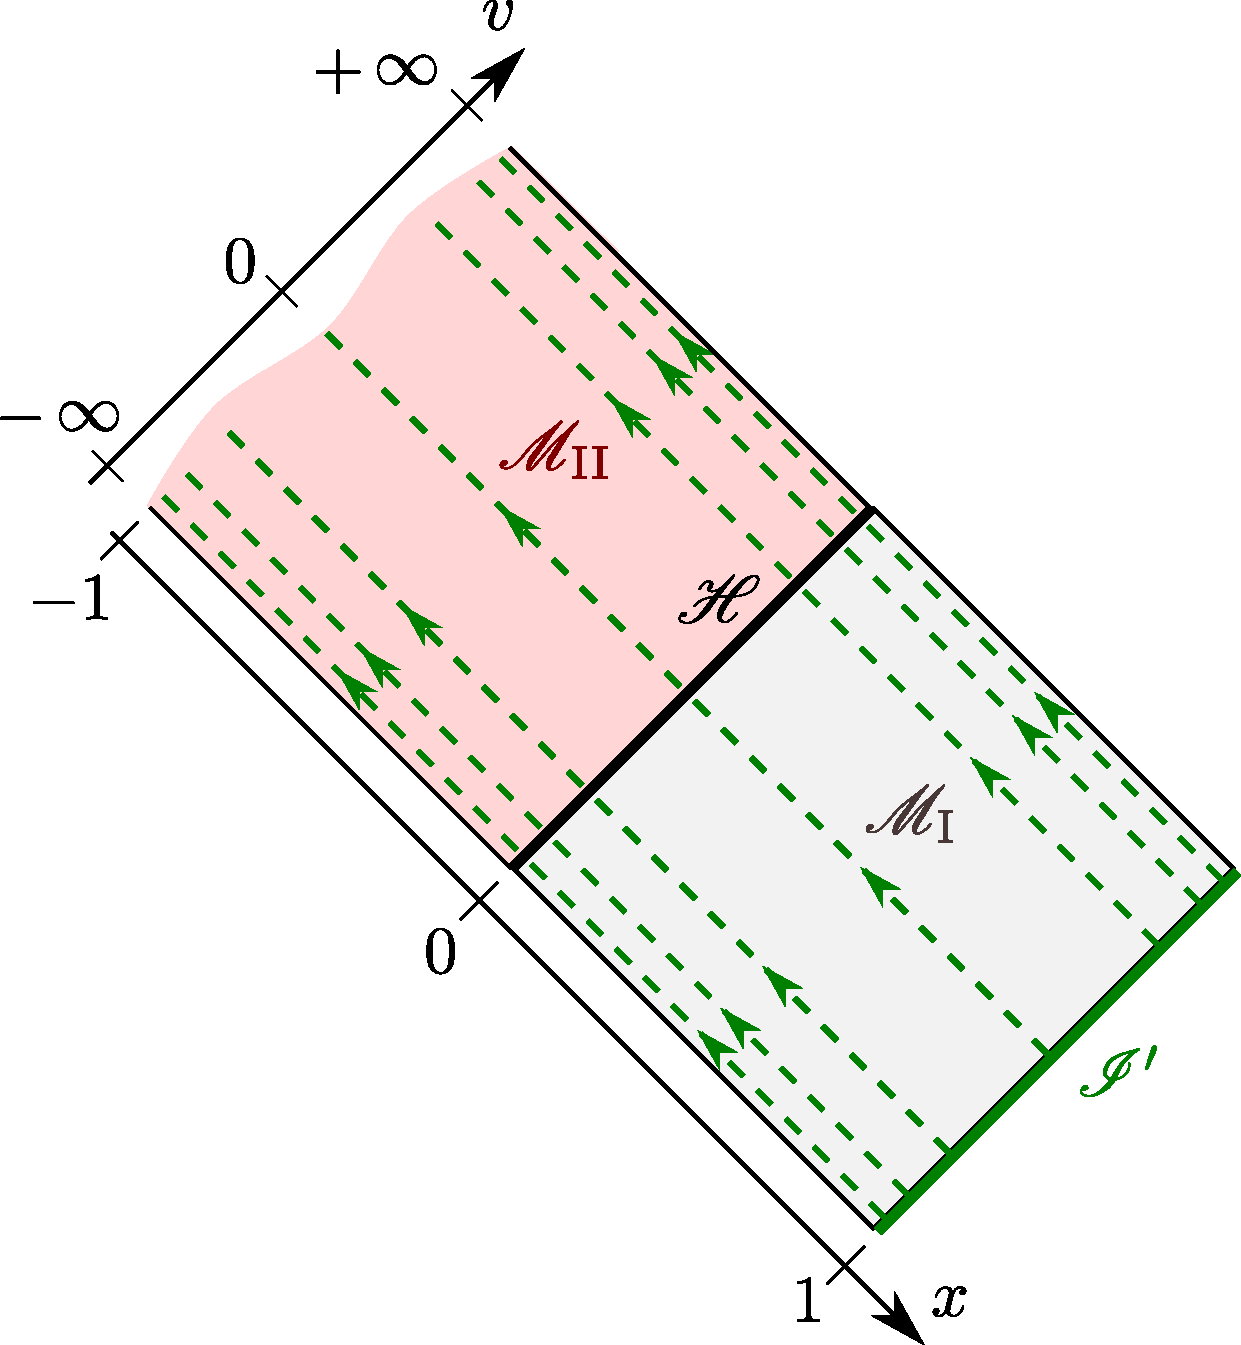
\includegraphics[width=0.5\textwidth]{sch_conf_compl1.pdf}}
\caption[]{\label{f:sch:conf_compl1} \footnotesize
Manifold with boundary
$\M' = \M_{\rm II}\cup\Hor\cup\M_{\rm I}\cup\scri'$, drawn in terms of
the coordinates $x$ and (a compactified version of) $v$.
The dashed lines are the ingoing radial null geodesics (as in Fig.~\ref{f:sch:rad_null_geod_EF}), the arrows marking the future orientation.}
\end{figure}


It would be satisfactory though to check that $\M_{\rm II}$ fulfills the
formal definition of a black hole region that we have given in
Sec.~\ref{s:glo:def_BH}.
The first step is to define a conformal
completion at null infinity $(\tilde{\M},\w{\tilde{g}})$ of
the Schwarzschild spacetime $(\M, \w{g})$, as defined by Eq.~(\ref{s:sch:def_Schwarz_spacetime}).
To this aim, let us start from the null ingoing Eddington-Finkelstein
coordinates $(x^{\hat{\alpha}})=(v,r,\th,\ph)$ introduced in Sec.~\ref{s:sch:EF_coord}; they
cover entirely $\M$ and the metric tensor $\w{g}$
is expressed in terms of them by Eq.~(\ref{e:sch:Schwarz_metric_NIEF}).
Performing the change of coordinates
$(x^{\hat{\alpha}})=(v,r,\th,\ph)\mapsto (x^{\alpha'}) = (v,x,\th,\ph)$
with
\be \label{e:sch:x_r}
    x = 1 - \frac{2m}{r} \iff r = \frac{2m}{1-x}, \qquad x\in (-\infty, 1),
\ee
we deduce from (\ref{e:sch:Schwarz_metric_NIEF}) that
\be
        \w{g} =
            -x \, \dd v^2
            +\frac{4 m}{(1-x)^2} \, \dd v \, \dd x
        + \frac{4 m^2}{(1-x)^2}  \left( \dd\th^2 + \sin^2\th\, \dd\ph^2 \right) .
\ee
Defining
\be \label{e:sch:Omega_x_r}
    \Omega := 1-x = \frac{2m}{r} ,
\ee
we may rewrite the metric tensor as
\be
    \w{g} = \Omega^{-2} \w{\tilde{g}} ,
\ee
with
\be \label{e:sch:tilde_g_x_v}
    \w{\tilde{g}}  = - x(1-x)^2 \, \dd v^2
            +4 m \, \dd v \, \dd x
        + 4 m^2 \left( \dd\th^2 + \sin^2\th\, \dd\ph^2 \right) .
\ee
Since $(v,x,\th,\ph)$ is a global coordinate system on $\M$
(up to the trivial coordinate singularities of $(\th,\ph)$), we can
identify $\M$ with the following open subset of $\R^2\times\SS^2$:
\be \label{e:sch:M_subset_R2_S2}
    \M = \R \times (-\infty,1) \times \SS^2,
\ee
with $v$ spanning $\R$, $x$ spanning $(-\infty,1)$ and $(\th,\ph)$
spanning $\SS^2$.
We can then extend $\M$ to the manifold with boundary\footnote{Cf. Sec.~\ref{s:bas:manif_boundary} for the definition of a \emph{manifold with boundary}.}
\be
    \M' :=  \R \times (-\infty,1] \times \SS^2 .
\ee
Notice the change $(-\infty,1) \rightarrow (-\infty,1]$ with respect
to (\ref{e:sch:M_subset_R2_S2}), which means
that $x=1$ is an allowed value on $\M'$; it actually defines the boundary of
$\M'$, $\scri'$ say.
According to (\ref{e:sch:x_r}),
$\scri'$ corresponds to $r\rightarrow +\infty$.
A view of the manifold $\M'$ is
provided in Fig.~\ref{f:sch:conf_compl1}.
We note that the conformal metric (\ref{e:sch:tilde_g_x_v}) can be extended
to the boundary $\scri'$, yielding a regular metric. Indeed, the determinant of
the metric components (\ref{e:sch:tilde_g_x_v}) is
\[
    \det\left({\tilde{g}}_{\alpha'\beta'}\right) = - 64 m^6 \sin^2\th ,
\]
which does not vanish at $x=1$ (except at the trivial coordinate singularity
$\th=0$ or $\th=\pi$), showing that $\tilde{\w{g}}$ is a non-degenerate
symmetric bilinear form at $\scri'$ and hence a well-defined metric on all
$\M'$.
Furthermore
we have $\Omega >0$ on $\M$ and $\Omega=0$ at $\scri'$ [set $x=1$ in Eq.~(\ref{e:sch:Omega_x_r})], as well as
\be
    \dd \Omega = - \dd x \not = 0 .
\ee
Hence $(\M',\w{\tilde{g}})$ obeys all the conditions
listed in Sec.~\ref{s:glo:conf_compl} to be a \emph{conformal completion at infinity}
of $(\M,\w{g})$.
However, it is not adapted to the black hole definition given in Sec.~\ref{s:glo:def_BH}. Indeed
$\scri'$ does not include any future infinity ($\scri^+$). Actually, $\scri'$ is
entirely a past infinity: a generic point of $\scri'$ has coordinates
$(v,x,\th,\ph) = (v_0,1,\th_0,\ph_0)$ and is the past end point of the
ingoing radial null geodesic defined by
$(v,\th,\ph) = (v_0,\th_0,\ph_0)$.
Therefore, we shall extend $\M'$ to include some $\scri^+$ part.
To achieve this, we shall construct $\scri^+$ as the set of endpoints of the
\emph{outgoing} radial null geodesics in $\M_{\rm I}$. In terms of
the null ingoing Eddington-Finkelstein coordinates $(v,r,\th,\ph)$,
the equation of these geodesics is obtained by combining (\ref{e:sch:outgoing_null_geod_EF}) and (\ref{e:sch:ingoing_null_geod_EF}):
\be \label{e:sch:v_r_u}
    v = 2 r + 4 m \ln \left| \frac{r}{2m} - 1 \right| + u ,
\ee
where $u\in\R$ is a constant parameter along a given geodesic.
We notice that on $\M_{\rm I}$, we may use $(x^{\check{\alpha}}) = (u,r,\th,\ph)$ as a coordinate
system, naturally called the \defin{null outgoing Eddington-Finkelstein coordinates}\index{Eddington-Finkelstein!coordinates}\index{null!outgoing Eddington-Finkelstein coordinates}. Since (\ref{e:sch:v_r_u}) implies
\[
    \dd v = \dd u + \frac{2}{1-2m/r}\, \dd r,
\]
we easily deduce from (\ref{e:sch:Schwarz_metric_NIEF}) the metric components
in these coordinates:
\be \label{e:sch:g_u_r}
    \w{g} = -\left( 1 - \frac{2 m}{r} \right)\, \dd u^2
            - 2 \, \dd u \, \dd r
        + r^2 \left( \dd\th^2 + \sin^2\th\, \dd\ph^2 \right) .
\ee
\begin{remark}
Contrary to $(v,r,\th,\ph)$, the coordinates $(u,r,\th,\ph)$ do not cover
all $\M = \M_{\rm IEF}$, but only $\M_{\rm I}$. This is graphically
evident from
Fig.~\ref{f:sch:rad_null_geod_EF}, where the outgoing radial null geodesics
$\Li^{\rm out,I}_{(u,\th,\ph)}$
accumulate on $\Hor$ as $u\rightarrow +\infty$
from the $\M_{\rm I}$ side.
\end{remark}

\begin{figure}
\centerline{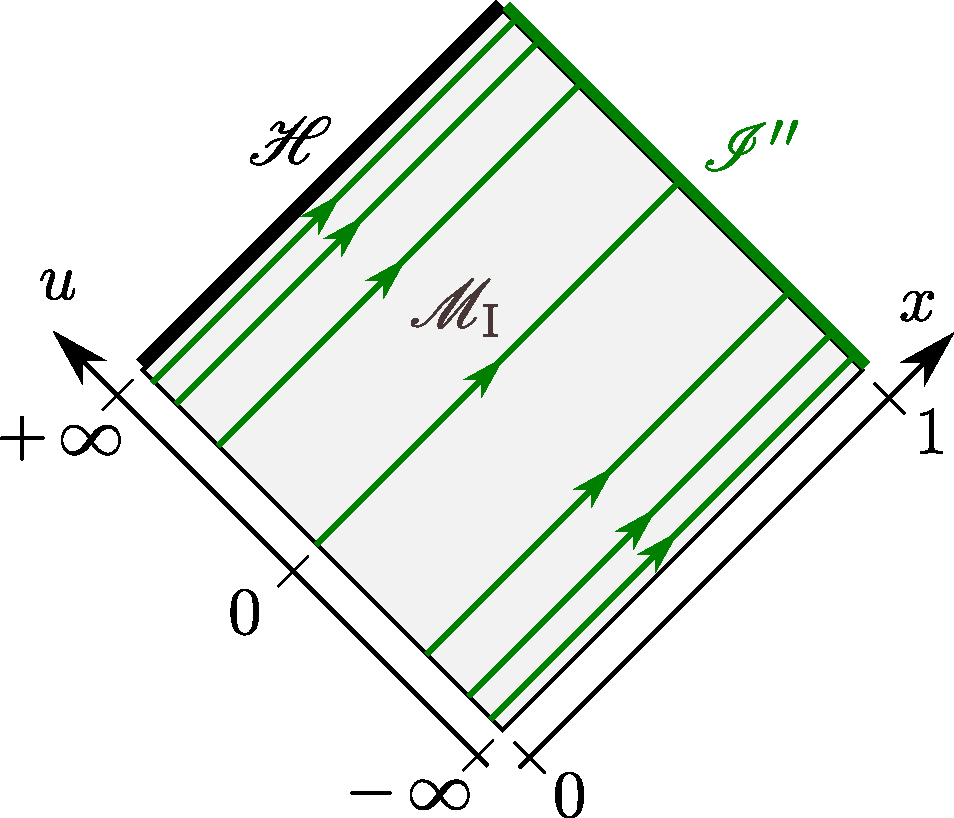
\includegraphics[width=0.4\textwidth]{sch_conf_compl2.pdf}}
\caption[]{\label{f:sch:conf_compl2} \footnotesize
Manifold with boundary
$\M''_{\rm I} = \M_{\rm I}\cup\scri''$, drawn in terms of
the coordinates $x$ and (a compactified version of) $u$.
The green solid lines are the outgoing radial null geodesics (as in Fig.~\ref{f:sch:rad_null_geod_EF}), the arrows marking the future orientation.
Note that $\Hor$, which is drawn on this figure, is not part of $\M''_{\rm I}$.}
\end{figure}

On $\M_{\rm I}$, let us perform the change of coordinates
$(x^{\check{\alpha}}) = (u,r,\th,\ph) \rightarrow (x^{\alpha''}) = (u,x,\th,\ph)$,
where $x$ is related to $r$ by the same formula as (\ref{e:sch:x_r}),
except that on $\M_{\rm I}$, $x$'s range is $(0,1)$ only.
We deduce from (\ref{e:sch:g_u_r}) and (\ref{e:sch:x_r})
the expression of $\w{g}$ in terms of the coordinates $(u,x,\th,\ph)$:
\be
        \w{g} = -x \, \dd u^2
            -\frac{4 m}{(1-x)^2} \, \dd u \, \dd x
        + \frac{4 m^2}{(1-x)^2}  \left( \dd\th^2 + \sin^2\th\, \dd\ph^2 \right) .
\ee
Let us identify $\M_{\rm I}$ with the following open subset of
$\R^2\times \SS^2$:
\be
    \M_{\rm I} = \R \times (0,1) \times \SS^2 ,
\ee
with $u$ spanning $\R$, $x$ spanning $(0,1)$ and $(\th,\ph)$
spanning $\SS^2$. Similarly to what we did above for $\M$, we may then
extend $\M_{\rm I}$ to the manifold with boundary
\be
    \M''_{\rm I} :=  \R \times (0,1] \times \SS^2 .
\ee
The boundary of $\M''_{\rm I}$, $\scri''$ say, lies at $x=1$
(cf. Fig.~\ref{f:sch:conf_compl2}). It shall not be
confused with the boundary of $\M_{\rm I}$ as a submanifold of $\M'$, which is
$\scri'$. The difference arises from the fact that $u$ diverges (to $-\infty$)
when one approaches $\scri'$ in $\M'$, so that $u$ cannot be used as a
coordinate on $\M'$. This is clear on the relation (\ref{e:sch:v_r_u})
between $u$, $v$ and $r$, which, once re-expressed in terms of $x$, becomes
\be \label{e:sch:u_v_x}
    u = v - 4m\left[ \frac{1}{1-x} + \ln\left( \frac{x}{1-x} \right) \right].
\ee
For a fixed value of $v$ in $\M'$, this relation yields indeed diverging values of
$u$ at two places:
\begin{itemize}
\item $x\rightarrow 0^+$ (the horizon $\Hor$): $u\rightarrow +\infty$;
\item $x\rightarrow 1^-$ (the boundary $\scri'$): $u\rightarrow -\infty$.
\end{itemize}
Reciprocally, for a fixed value of $u$, relation~(\ref{e:sch:u_v_x})
implies that $v$ diverges (to $+\infty$) when $x\rightarrow 1^-$, which shows that
$\scri''$ is not included in $\M'$.

The conformal metric $\w{\tilde{g}}$ on $\M''_{\rm I}$ is given by
\be \label{e:sch:tilde_g_x_u}
     \w{\tilde{g}} =
            - x(1-x)^2 \, \dd u^2
            - 4 m \, \dd u \, \dd x
        + 4 m^2 \left( \dd\th^2 + \sin^2\th\, \dd\ph^2 \right) .
\ee
We notice that it is regular and non-degenerate in all $\M''_{\rm I}$,
including on $\scri''$ ($x=1$), and that on the submanifold $\M_{\rm I}$, it is related to the physical metric $\w{g}$ by $\w{\tilde{g}} = \Omega^2 \w{g}$, with the
scalar field $\Omega$ taking the same expression in terms of $x$ as
that introduced in Eq.~(\ref{e:sch:Omega_x_r}): $\Omega=1-x$.


The conformal completion of $(\M,\w{g})$ including both $\scri'$ (as $\scri^-$)
and $\scri''$ (as $\scri^+$) is constructed as follows. Let
\be
    \tilde{\M} = \M' \cup \M''_{\rm I} .
\ee
We endow $\tilde{\M}$ with two coordinate charts:
\be
    \begin{array}{rccl}
        \Phi_1: & \M' & \longrightarrow &   \R \times (-\infty,1] \times \SS^2 \\
        & p & \longmapsto & (v,x,\th,\ph) \\[1ex]
    \end{array}
    \qquad\mbox{and}\qquad
    \begin{array}{rccl}
        \Phi_2: & \M''_{\rm I}  & \longrightarrow & \R \times (0,1] \times \SS^2 \\
        & p & \longmapsto & (u,x,\th,\ph)
    \end{array}
\ee
and define the intersection of the two chart codomains:
\be
   \M' \cap  \M''_{\rm I} = \{ p \in \M',\  x(p) \in (0,1) \}
      = \{ p \in \M''_{\rm I},\  x(p) \in (0,1) \} ,
\ee
along with the transition map implementing (\ref{e:sch:u_v_x}):
\be
    \begin{array}{rccl}
        \Phi_2 \circ \Phi_1^{-1}: & \R \times (0,1) \times \SS^2  & \longrightarrow & \R \times (0,1) \times \SS^2 \\
        & (v,x,\th,\ph) & \longmapsto & \left(u = v - 4m\left[ \frac{1}{1-x} + \ln\left( \frac{x}{1-x} \right) \right],\; x,\; \th,\; \ph \right) ,
    \end{array}
\ee
The above construction makes $\tilde{\M}$ a manifold with boundary
(cf. Fig.~\ref{f:sch:conf_compl_final}), the boundary
being
\be
    \scri = \scri^+ \cup \scri^- ,
\ee
with
\be
    \scri^+ := \{ p \in \M''_{\rm I}, \  x(p) = 1 \}
     \qquad\mbox{and}\qquad
    \scri^- := \{ p \in \M', \ x(p) = 1 \} .
\ee

\begin{figure}
\centerline{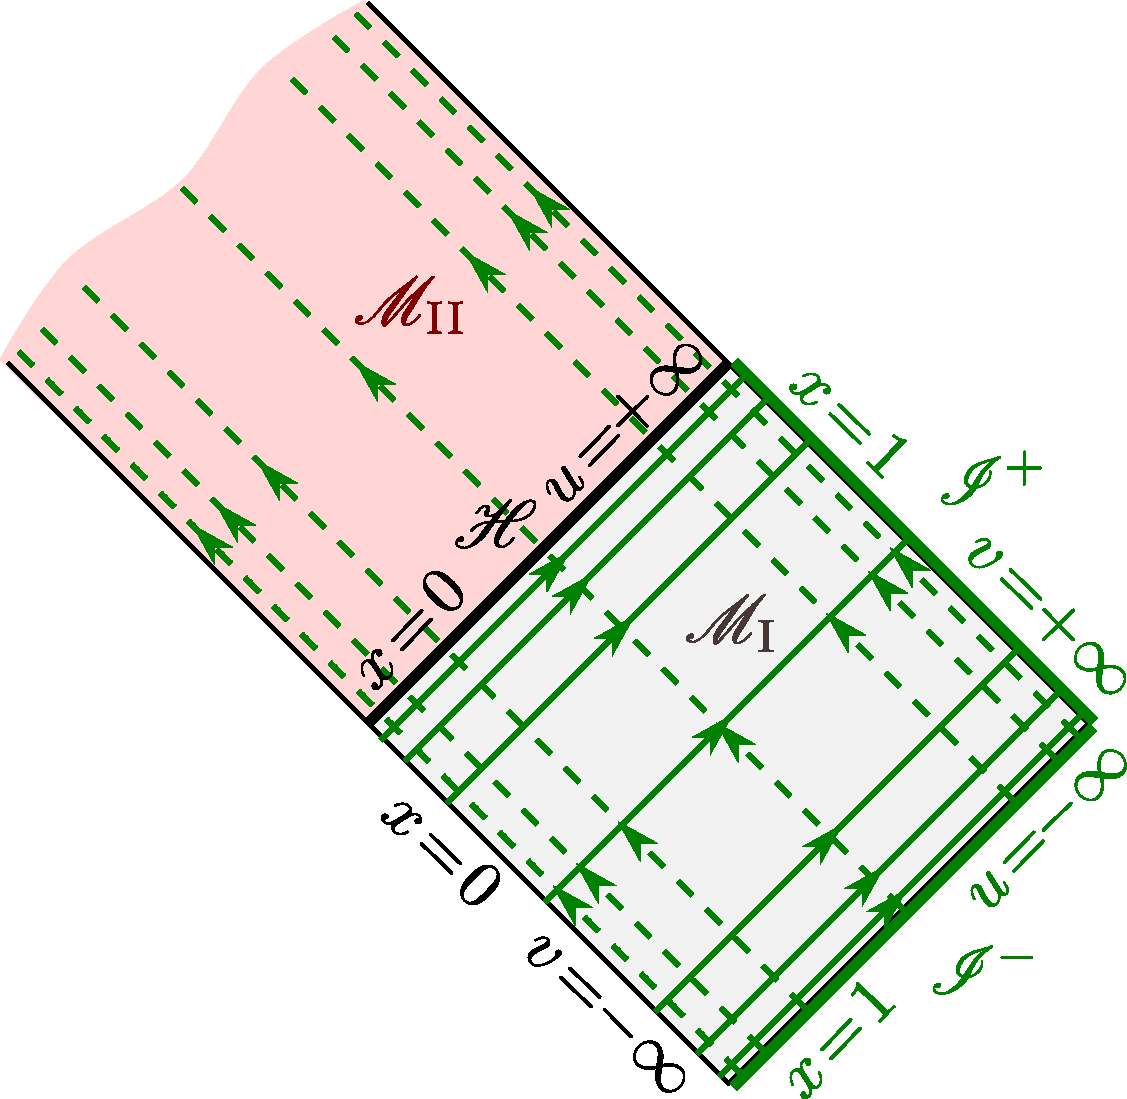
\includegraphics[width=0.5\textwidth]{sch_conf_compl_final.pdf}}
\caption[]{\label{f:sch:conf_compl_final} \footnotesize
Schematic view of the manifold with boundary $\tilde{\M}$, which defines
a conformal completion at null infinity of Schwarzschild spacetime
$(\M,\w{g})$.
\textsl{NB:} contrary to Figs.~\ref{f:sch:conf_compl1} and~\ref{f:sch:conf_compl2}, this figure is not drawn on some specific coordinate system.
As in Figs.~\ref{f:sch:rad_null_geod_EF}, \ref{f:sch:conf_compl1} and~\ref{f:sch:conf_compl2},
the green solid (resp. dashed) lines are the outgoing (resp. ingoing) radial null geodesics, the arrows marking the future orientation.
}
\end{figure}


We then endow $\tilde{\M}$ with a Lorentzian metric $\w{\tilde{g}}$, whose
expression is given by (\ref{e:sch:tilde_g_x_v}) on $\M'$ and
by (\ref{e:sch:tilde_g_x_u}) on $\M''_{\rm I}$.
By construction, $(\tilde{\M},\w{\tilde{g}})$ is then a conformal completion at null
infinity of the Schwarzschild spacetime $(\M,\w{g})$, the conformal factor
$\Omega$ being given by (\ref{e:sch:Omega_x_r}) in both
charts $(\M',\Phi_1)$ and $(\M''_{\rm I},\Phi_2)$: $\Omega = 1 -x$.
In particular, it is clear that no past-directed causal curve originating in
$\M$ intersects $\scri^+$ and that no future-directed causal curve originating in
$\M$ intersects $\scri^-$. We also check immediately that $\scri^+$ and $\scri^-$
are null hypersurfaces with respect to the metric $\w{\tilde{g}}$:
both hypersurfaces are defined by $x=1$, so that the induced metric on them,
as
deduced from (\ref{e:sch:tilde_g_x_v}) and
(\ref{e:sch:tilde_g_x_u}), is
\be
    \left. \w{\tilde{g}} \right| _{\scri^\pm} = 4 m^2 \left(
        \dd \th^2  + \sin^2\th \, \dd \ph^2 \right) ,
\ee
which is clearly degenerate (along the $u$ direction for $\scri^+$
and along the $v$ direction for $\scri^-$).

As it is clear from Fig.~\ref{f:sch:conf_compl_final}, $\M_{\rm I}$
is the interior of the causal past of $\scri^+$ within $\M$:
\be
    \M_{\rm I} = \mathrm{int}\left( J^-(\scri^+)\cap\M \right).
\ee
In view of the formal definition (\ref{e:glo:def_BH}), we conclude:
\begin{prop}[black hole region in Schwarzschild spacetime]
The Schwarzschild spacetime $(\M=\M_{\rm IEF}, \w{g})$
has a black hole region $\mathscr{B}$, the interior
of which is $\M_{\rm II}$; the event horizon is nothing but the
Schwarzschild horizon $\Hor$ discussed in Sec.~\ref{s:sch:Schwarz_hor}.
\end{prop}

\begin{remark}
As stated at the beginning of this section, the null character of the boundary
$\Hor$ between $\M_{\rm I}$ and $\M_{\rm II}$ and the fact that
$\M_{\rm II}$ never intersect the asymptotically flat region $r\rightarrow +\infty$,
was sufficient to claim that $\M_{\rm II}$ represents what by any means should be
called a \emph{black hole region}.
Therefore, we can view the above demonstration more as a ``sanity check''
of the formal definition of a black hole given in Sec.~\ref{s:glo:def_BH}:
this definition would not have been acceptable if it would not
apply to the Schwarzschild spacetime.
\end{remark}

\begin{remark}
The above construction of the conformal completion at null infinity
$(\tilde{\M},\w{\tilde{g}})$ involves two coordinate charts,
$(v,x,\th,\ph)$ and $(u,x,\th,\ph)$, with two different
domains, $\M'$ and $\M''_{\rm I}$.
As will be discussed in Chap.~\ref{s:max},
one may construct a conformal completion
with a single chart, as in the Minkowski case, but its relation with
the coordinates introduced so far is quite involved.
In particular the standard compactification of Kruskal-Szekeres coordinates,
which is used in many textbooks to construct the Carter-Penrose diagram
of Schwarzschild spacetime, does \emph{not} provide any
conformal completion, as it will be discussed in
Sec.~\ref{s:max:discus_hUhV}.
\end{remark}

